\documentclass[12pt,a4paper,oneside]{book}
\usepackage{a4wide}                     % Iets meer tekst op een bladzijde
\usepackage[dutch,english]{babel}       % Voor nederlandstalige hyphenatie (woordsplitsing)
\usepackage{amsmath}                    % Uitgebreide wiskundige mogelijkheden
\usepackage{amssymb}                    % Voor speciale symbolen zoals de verzameling Z, R...
\usepackage{url}                        % Om url's te verwerken
\usepackage{graphicx}                  % Om figuren te kunnen verwerken
\usepackage[small,bf]{caption}    % Om de captions wat te verbeteren
\usepackage{xspace}                     % Magische spaties na een commando
\usepackage[utf8]{inputenc}           	% Om niet ascii karakters rechtstreeks te kunnen typen
\usepackage{float}                      % Om nieuwe float environments aan te maken. Ook optie H!
\usepackage{flafter}                    % Opdat floats niet zouden voorsteken
\usepackage{listings}                   % Voor het weergeven van letterlijke text en codelistings
\usepackage{marvosym}                   % Om het euro symbool te krijgen
\usepackage{textcomp}                   % Voor onder andere graden celsius
\usepackage{fancyhdr}                   % Voor fancy headers en footers.
\usepackage{graphics}					% Om figuren te verwerken.
\usepackage[nottoc]{tocbibind} 			% Bibliografie in ToC; zie tocbibind.dvi
%\usepackage{pstricks}
\usepackage{longtable}
\usepackage{pdfpages}  					% pdf pagina's importeren
\usepackage[numbers]{natbib}			% Extra citeer mogelijkheden
\usepackage{parskip}					% Geen indentatie bij begin paragraaf
\usepackage[hang,flushmargin,bottom]{footmisc} % Voetnoten beter weergeven (niet laten splitsen)
\usepackage{enumitem} 					%Betere opsommingen
\usepackage{sidecap}  					%Caption lang
\usepackage[toc,page]{appendix} 		%Appendices toevoegen
\usepackage{tikz}						%Toevoegen van tikz figuren
\usepackage{pgfplots}					%Grafieken plotten in tikz figuren
\usepackage{amsmath}
\usepackage{tikzscale}
\usepackage{environ}
\usepackage{authblk} 
\usetikzlibrary{arrows}
\usepackage{wrapfig}					%Figuren wrappen
\usepackage{subfig}                     %Figuren naast elkaar floaten


\interfootnotelinepenalty=10000

\newcommand{\npar}{\par \vspace{2.3ex plus 0.3ex minus 0.3ex} \noindent}	% Om witruimte te krijgen tussen paragrafen
\graphicspath{{figuren/}}               % De plaats waar latex zijn figuren gaat halen.
%\usepackage[bf]{caption2}				% Mooiere captions
\usepackage[a4paper,plainpages=false]{hyperref}    % Om hyperlinks te hebben in het pdfdocument.

\newcommand{\command}[1]{\lstinline[basicstyle=\tt]{#1}\xspace} %Voor commando's
\hyphenation{tijd-as audio-stream} 							% Splitsing van woorden

\renewcommand{\chaptermark}[1]{\markright{\MakeUppercase{#1}}}
\renewcommand{\sectionmark}[1]{\markright{\thesection~#1}}

\newcommand{\headerfmt}[1]{\textsl{\textsf{#1}}}
\newcommand{\headerfmtpage}[1]{\textsf{#1}}

\fancyhf{}
\fancyhead[LE,RO]{\headerfmtpage{\thepage}}
\fancyhead[LO]{\headerfmt{\rightmark}}
\fancyhead[RE]{\headerfmt{\leftmark}}
\renewcommand{\headrulewidth}{0.5pt}
\renewcommand{\footrulewidth}{0pt}

\fancypagestyle{plain}{ % eerste bladzijde van een hoofdstuk
	\fancyhf{}
	\fancyhead[LE,RO]{\headerfmtpage{\thepage}}
	\fancyhead[LO]{\headerfmt{\rightmark}}
	\fancyhead[RE]{\headerfmt{\leftmark}}
	\renewcommand{\headrulewidth}{0.5pt}
	\renewcommand{\footrulewidth}{0pt}
}

\renewcommand{\lstlistoflistings}{\begingroup
	\tocfile{\lstlistlistingname}{lol}
	\endgroup}


% anderhalve interlinie (opm: titelblad gaat uit van 1.5)
\renewcommand{\baselinestretch}{1.5}


%Pdf instellen, links, meta info
\hypersetup {
	pdfauthor = {Ward Van Assche},
	pdftitle = {Realtime signaal synchronisatie	met accoustic fingerprinting},
	pdfsubject = {Masterproef ingediend tot het behalen van de academische graad van Master of Science in de industriële wetenschappen: informatica, juni 2016},
	colorlinks = False,
%	pdfborder = {0 0 0}
}

%Titels wijzigen in correcte Nederlandse term
\renewcommand\lstlistlistingname{Lijst van codefragmenten}
\renewcommand\lstlistingname{Codefragment}
\addto{\captionsdutch}{\renewcommand{\bibname}{Referentielijst}}

\begin{document}
\selectlanguage{dutch}

%officieel Plato titelblad
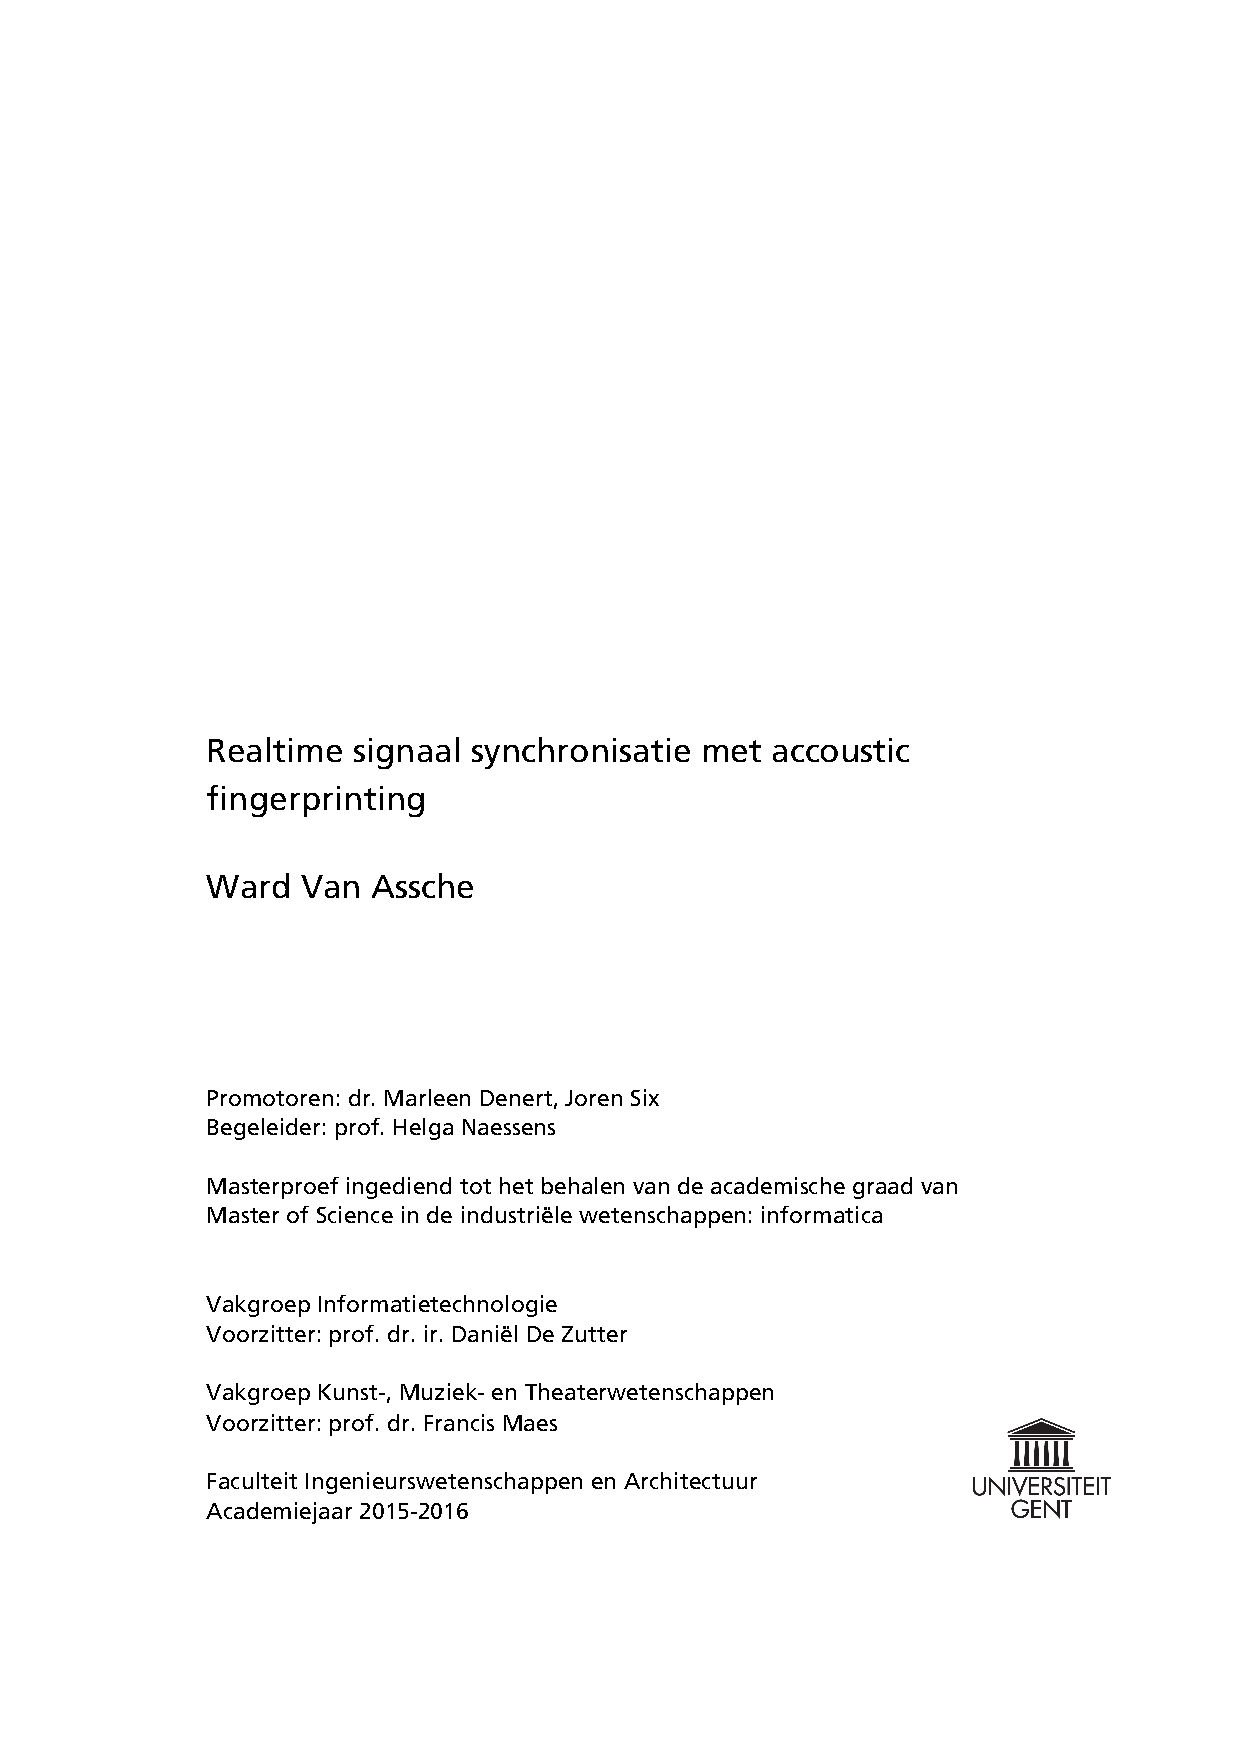
\includepdf[pages=-]{./titelblad.pdf}

% titelblad (voor kaft)
%  Titelblad

% Opmerking: gaat uit van een \baselinestretch waarde van 1.5 (die moet
% ingesteld worden voor het begin van de document environment)

\begin{titlepage}

\setlength{\hoffset}{-1in}
\setlength{\voffset}{-1in}
\setlength{\topmargin}{1.5cm}
\setlength{\headheight}{0.5cm}
\setlength{\headsep}{1cm}
\setlength{\oddsidemargin}{3cm}
\setlength{\evensidemargin}{3cm}
\setlength{\footskip}{1.5cm}
\enlargethispage{1cm}
% \textwidth en \textheight hier aanpassen blijkt niet te werken

\fontsize{12pt}{14pt}
\selectfont

\begin{center}


\includegraphics[height=2cm]{fig/ruglogo}

\vspace{0.5cm}

Faculteit Ingenieurswetenschappen en Architectuur\\
Vakgroep Informatietechnologie\\
Voorzitter: Prof.~Dr.~Ir.~Dani\"{e}l De Zutter

\vspace{3.5cm}

\fontseries{bx}
\fontsize{17.28pt}{21pt}
\selectfont

Realtime signaal synchronisatie \\
met accoustic fingerprinting

\fontseries{m}
\fontsize{12pt}{14pt}
\selectfont

\vspace{.6cm}

door 

\vspace{.4cm}

Ward Van Assche

\vspace{3.5cm}

Promotoren: Dr.~Marleen Denert, Joren Six\\
Scriptiebegeleider: Prof.~Helga Naessens\\

\vspace{2cm}

Masterproef ingediend tot het behalen van de academische graad van\\
Master of Science in de industri\"{e}le wetenschappen: informatica

\vspace{1cm}

Academiejaar 2015--2016

\end{center}
\end{titlepage}


% lege pagina (!!)

% titelblad (!!)

% geen paginanummering tot we aan de inhoudsopgave komen
\pagestyle{empty}

% voorwoord met dankwoord en toelating tot bruikleen (ondertekend)
%  Voorwoord (dankwoord) en toelating tot bruikleen

\newpage

\noindent \textbf{\huge Voorwoord}

\vspace{1.5cm}

\noindent

Zonder hulp van buitenaf zou ik er nooit in geslaagd zijn om mijn masterproef tot een goed einde te brengen. Daarom wil ik verschillende mensen bedanken die een grote rol gespeeld in één of meerdere fases van dit eindwerk.

Eerst en vooral wil ik mijn externe promotor, Joren Six, bedanken voor het vertrouwen en de ondersteuning die hij mij tijdens het uitwerken van deze masterproef heeft gegeven. De kennis en inzicht die ik van hem heb meegekregen op vlak van digitale audio (en alles wat ermee te maken heeft) zal mij zeker bijblijven. Ik vond het ontzettend leerrijk om mijn interesse in muziek en geluid te kunnen combineren met mijn opleiding informatica.

Verder wil ik ook mijn interne promotor, Marleen Denert, bedanken voor het opvolgen en nalezen van mijn thesis. Haar opbouwende kritiek was van onschatbare waarde.

Ten slotte wil ik ook mijn ouders, zusje en vrienden bedanken die mij altijd gesteund hebben tijdens mijn opleiding tot industrieel ingenieur.

En uiteraard wil ik ook u, de lezer, bedanken voor de interesse in mijn onderzoek. Ik wens u veel leesplezier.

\addvspace{2.5cm}

\noindent Ward Van Assche, juni 2016\newpage

\noindent \textbf{\huge Toelating tot bruikleen}

\vspace{1.5cm}

\noindent
``De auteur geeft de toelating deze scriptie voor consultatie beschikbaar
te stellen en delen van de scriptie te kopi\"eren voor persoonlijk
gebruik.\\
Elk ander gebruik valt onder de beperkingen van het auteursrecht,
in het bijzonder met betrekking tot de verplichting de bron uitdrukkelijk
te vermelden bij het aanhalen van resultaten uit deze scriptie.''

\addvspace{4cm}

\noindent Ward Van Assche, juni 2016


% overzicht
%  Overzichtsbladzijde met samenvatting

\newpage

{
\setlength{\baselineskip}{14pt}
\setlength{\parindent}{0pt}
\setlength{\parskip}{8pt}

\begin{center}

\noindent \textbf{\huge
Realtime signaal synchronisatie\\[8pt]
met accoustic fingerprinting
}

door 

Ward Van Assche

Masterproef ingediend tot het behalen van de academische graad van\\
Master of Science in de industriële wetenschappen: informatica

Academiejaar 2015--2016

Promotoren: Dr.~Marleen Denert, Joren Six\\
Scriptiebegeleider: Prof.~Helga Naessens

Faculteit Ingenieurswetenschappen en Architectuur\\
Universiteit Gent

Vakgroep Informatietechnologie\\
Voorzitter: Prof.~Dr.~Ir.~Dani\"{e}l De Zutter


\end{center}

\section*{Samenvatting}

% TODO: samenvatting schrijven

\textit{Todo: samenvatting schrijven}




\section*{Trefwoorden}

% TODO: trefwoorden

synchronisatie, realtime, datastromen, musicologie, accoustic fingerprinting

}
\newpage % strikt noodzakelijk om een header op deze blz. te vermijden


% abstract pdf toevoegen
\addcontentsline{toc}{chapter}{Extended abstract}
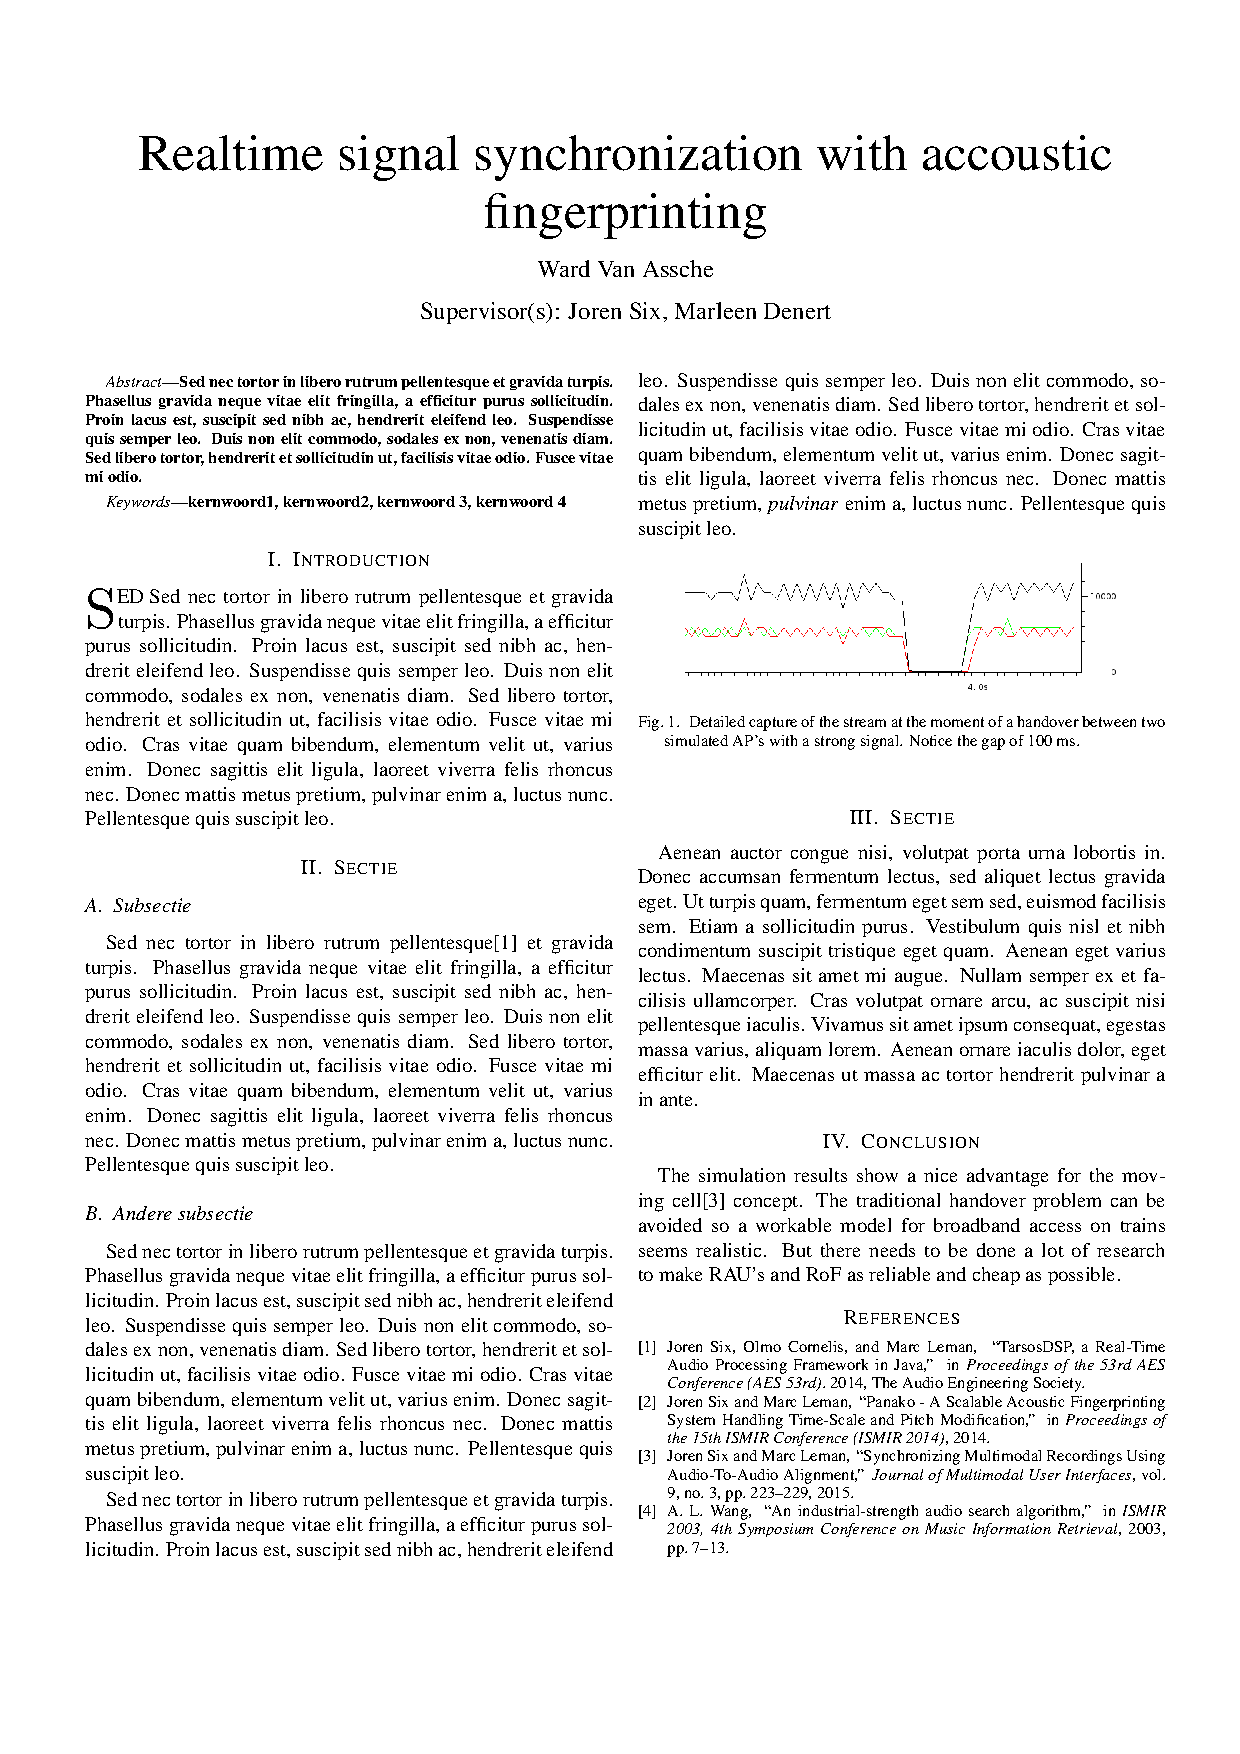
\includepdf[pages=-]{../abstract/abstract.pdf}
\pagestyle{fancy}

\frontmatter

% inhoudstafel
\tableofcontents

% afkortingen
\chapter{Gebruikte afkortingen}
\begin{flushleft}
	\renewcommand{\baselinestretch}{1.5}
	\small\normalsize
	\begin{longtable}{ll}
		IPEM				&  Instituut voor Psychoakoestiek en Elektronische Muziek \\
		DSP					&  Digital Signal Processing \\
		FFT					&  Fast Fourier Transform \\
		SFT					&  Short Time Fourier Transform \\
		ECG					&  Elektrocardiogram \\
		DTW					&  Dynamic timewarping \\
		USB					&  Universal Serial Bus \\
		ADC					&  Analog-to-digital converter \\
		PCM					&  Pulse-code modulation \\
		UML					&  Unified Modeling Language
		
	\end{longtable}
\end{flushleft}

% hoofdstukken
\mainmatter

% hier worden de hoofdstukken ingevoegd (\includes)
\chapter{Introductie}
\label{introductie}

\section{Probleemschets}
\label{probleemschets}

Het probleem dat in deze masterproef zal worden onderzocht doet zich heel specifiek voor bij verschillende experimenten die aan het IPEM worden uitgevoerd. Dit is de onderzoeksinstelling van het departement musicologie aan Universiteit Gent. De focus van het IPEM ligt vooral op onderzoek naar de interactie van muziek op fysieke aspecten van de mens zoals dansen, sporten en fysieke revalidatie. \cite{ipem2016}

Om de relatie tussen muziek en beweging te onderzoeken worden er tal van experimenten uitgevoerd. Deze experimenten maken gebruik van allerhande sensoren om bepaalde gebeurtenissen om te zetten in analyseerbare data. 

Bij een klassiek experiment wordt onderzocht wat de invloed is van muziek op de lichamelijke activiteit van een persoon. Alle bewegingen worden geregistreerd met een videocamera en een accelerometer.

Hierbij moeten drie datastreams worden geanalyseerd: de videobeelden, de data van de accelerometer en de afgespeelde audio. Een  uitdaging hierbij is de synchronisatie van deze verschillende datastreams. Om een goede analyse mogelijk te maken is het zeer gewenst dat men exact weet (tot op de milliseconde nauwkeurig) wanneer een bepaalde gebeurtenis in een datastream zich heeft voorgedaan, zodat men deze gebeurtenis kan vergelijken met de gebeurtenissen in de andere datastreams. Door de verschillen in samplefrequentie en door de latencies die zich in elke opname kunnen voordoen is dit zeker geen sinecure. \cite{six2015multimodal}

Bij het IPEM maakt men gebruik van een systeem waarbij audio opnames het synchronisatieproces vereenvoudigen. Het principe werkt als volgt: men zorgt ervoor dat elke datastream gekoppeld is aan een perfect gesynchroniseerde audiostream, afkomstig van een opname van het omgevingsgeluid. In het voorgaande experiment is dit eenvoudig te verwezenlijken. Bij de videobeelden kan automatisch een audiospoor mee worden opgenomen. De accelerometer kan geplaatst worden op een microcontroller vergezeld van een kleine microfoon. Aangezien beide componenten zo dicht op de hardware geplaatst zijn is de latency tussen beide datastromen te verwaarlozen.\footnote{De latency van de audioverwerking op een \textit{Axoloti} microcontroller is vastgesteld op $0.333 ms$. Meer informatie: \url{http://www.axoloti.com/more-info/latency/}} De afgespeelde audio is uiteraard al een perfecte weergave van het omgevingsgeluid. Figuur \ref{syncsink-ui} toont een screenshot van het programma waarmee de synchronisatie op dit moment wordt uitgevoerd.

Na het uitvoeren van het experiment beschikt men dus over de gegevens van drie datastreams, waarbij er aan elke datastream een quasi perfect synchrone opname van het omgevingsgeluid is gekoppeld. Aangezien het experiment in één ruimte is uitgevoerd zijn de verschillende opnames van het omgevingsgeluid zeer gelijkend. Het probleem van de synchronisatie van de verschillende datastromen kan bijgevolg gereduceerd worden tot het synchroniseren van de verschillende audiostromen.

Door de typisch eigenschappen van geluid is het niet zo moeilijk om verschillende audiostreams te synchroniseren. Bij het IPEM heeft men een systeem ontwikkeld dat hiertoe in staat is.

Dit systeem heeft in de praktijk echter heel wat beperkingen. De grootste beperking is dat het synchronisatieproces pas kan worden uitgevoerd wanneer het experiment is afgelopen. Deze verwerking kan ook enkel handmatig uitgevoerd worden. De opgenomen audio- en databestanden moeten worden verzameld op een computer waarna vervolgens de latency tussen de audiostreams bepaald kan worden. Met behulp van deze latency kunnen de datastreams worden gesynchroniseerd. 

Voor de musicologen die deze experimenten uitvoeren is deze werkwijze veel te omslachtig. Daarom is een eenvoudiger realtime systeem om de synchronisatie uit te voeren zeer gewenst.

\begin{figure}[!h]
	\captionsetup{width=0.7\textwidth}
	\centering
	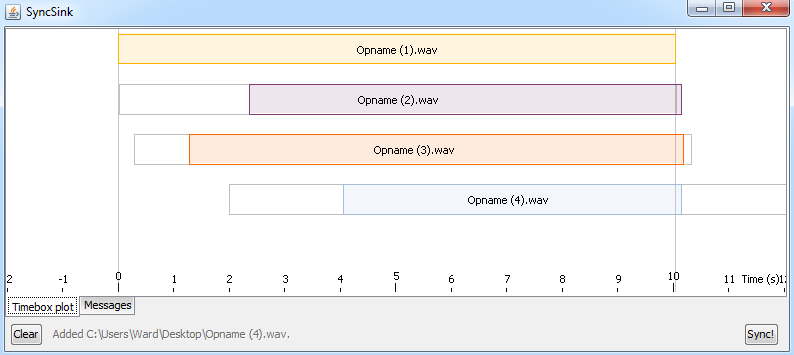
\includegraphics[width=0.5\textwidth]{syncsinc.png}
	\caption[Gebruikersinterface van SyncSink]{De gebruikersinterface van SyncSink: een programma waarin de opgenomen fragmenten gesleept kunnen worden na afloop van het experiment. Vervolgens wordt de latency berekend. Meer informatie is te vinden in artikel \cite{six2015multimodal}.}
	\label{syncsink-ui}
\end{figure}


Een ander probleem is dat de resultaten van het kruiscovariantie algoritme soms afwijkingen vertonen die moeilijk te verklaren zijn. De oorzaak hiervan zal worden onderzocht. Ook is het kruiscovariantie algoritme in vergelijking met het acoustic fingerprinting algoritme véél gevoeliger voor storingen en ruis, veroorzaakt door slechte opnames. Aangezien de opnameapparatuur (zeker op microcontrollers) bij de uit te voeren experimenten vaak van slechte kwaliteit is, is het belangrijk om de algoritmes voldoende robuust te maken zodat ze hier mee om kunnen.

\section{Digitale audio}

Het vervolg van deze scriptie onderstelt dat de lezer een basiskennis heeft inzake digitale audio. In deze inleiding worden de belangrijkste zaken hieromtrent uitgelegd.

Om geluidsgolven digitaal te kunnen verwerken moeten ze worden geconverteerd naar reeksen van discrete waarden. Deze omzetting gebeurt met een ADC: een analog-to-digital converter. De meeste ADC's maken gebruik van de PCM (pulse-code modulation) voorstelling van audio. Bij PCM wordt het analoge signaal op regelmatige tijdstippen gesampled en omgezet in discrete waarden. Figuur \ref{sampling} toont schematisch hoe dit in zijn werk gaat. PCM audio heeft verschillende parameters die een invloed hebben op de uiteindelijke kwaliteit van de audio. De belangrijkste parameters zijn de samplefrequentie (\textit{sampling rate}) en bitdiepte (\textit{bit depth}).

\begin{figure}[h!]
	\captionsetup{width=0.7\textwidth}
	\caption[Samplen van audio]{Samplen van een analoog audiosignaal in de vorm van een sinusgolf. Met toestemming overgenomen van artikel \cite{tarsosmanual2016}.}
	\begin{center}
		\advance\parskip0.3cm
		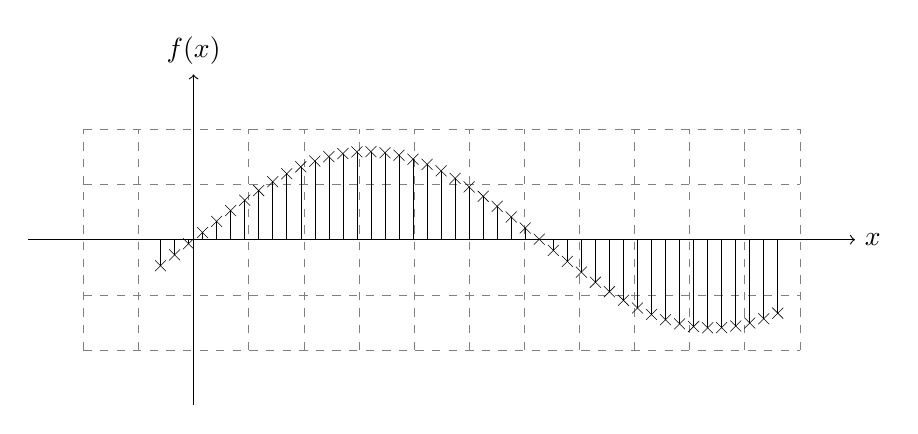
\begin{tikzpicture}[scale=1.4]
%grid
\draw[very thin,color=gray,step=.5cm,dashed] (-1,-1.0) grid (5.5,1);
\draw[->,color=black] (0,-1.5) -- (0,1.5)  node [above]{$f(x)$};
\draw[->,color=black] (-1.5,0) --  (6,0) node [right] {$x$};  
\draw[very thin,color=black,samples=45,domain=-0.3:5.3] 
plot[ycomb,thin,mark=x] (\x, { 0.8 * sin(\x r) });  
\end{tikzpicture}
	\end{center}
	\label{sampling}
\end{figure}

\subsubsection{Samplefrequentie}

De samplefrequentie bepaalt het aantal samples per seconde en wordt uitgedrukt in Hertz ($Hz$). Bij het bepalen van de samplefrequentie is het van belang om rekening te houden met het \textit{bemonsteringstheorema van Nyquist-Shannon}. Deze stelling zegt dat de samplefrequentie minstens dubbel zo hoog moet zijn dan de hoogste frequentie van de te converteren audio. Bij het samplen aan een lagere frequentie treedt informatieverlies op. Deze stelling wordt in detail besproken in het originele artikel \cite{nyquist1928certain} van \citeauthor{nyquist1928certain}.

Het menselijk oor is in staat om geluiden te detecteren tussen $20Hz$ en $20kHz$. Om informatieverlies bij het samplen van geluiden binnen dit bereik te voorkomen is het dus vereist om een minimale samplefrequentie te hanteren van $ 2 \times 20kHz $. De standaard samplefrequentie voor muziek is net iets hoger: $ 44.1kHz $.

De frequentie van de menselijke stem varieert tussen $ 30 Hz $ en $ 3000 Hz $. De minimale samplefrequentie voor het digitaliseren van een stemopname is dus $ 6kHz $. In de praktijk wordt meestal een minimum gehanteerd van $ 8kHz $.

\subsubsection{Bitdiepte}

De bitdiepte is het aantal bits waarmee elke gesamplede waarde wordt voorgesteld. Meestal wordt er gebruik gemaakt van 16 bit \textit{signed integers}.

De bitdiepte bepaalt het dynamische bereik van audio. Dit is de verhouding tussen het stilst en luidst mogelijk weer te geven volume. Deze verhouding, uitgedrukt in decibel, kan worden berekend met volgende formule: 
\begin{equation}
DR = 20 \cdot \log_{10} \left(\frac{2^Q}{1}\right) = (6.02 \cdot Q) dB
\end{equation}

In deze formule staat DR voor het dynamische bereik en Q voor de bitdiepte. Volgens deze formule heeft 16 bit audio een theoretisch dynamische bereik van ongeveer 96 dB. De werkelijke waarde kan hier echter van afwijken door filters die zijn ingebouwd in audiosystemen.

Bovenstaande informatie is gebaseerd op artikel \cite{tarsosmanual2016}, introductievideo \cite{xiph2016} en boek \cite{fries2005digital}.

\subsubsection{Weergave in software}

In computerprogramma's waarin digitale audio verwerkt wordt, wordt elke sample voorgesteld als een getal. Afhankelijk van de implementatie kan een 16 bit sample op verschillende manieren worden verwerkt. Enkele mogelijke voorstellingen: signed integer (-32768 tot 32767), unsigned integer (0 tot 65536) of floating point (-1 tot 1). 
In deze thesis en de bijhorende software wordt de floating point notatie gehanteerd.

\section{Evaluatiecriteria}
\label{evaluatie-criteria}

Het te ontwikkelen systeem moet voldoen aan heel wat vereisten. In deze sectie zullen de vereisten eenduidig geformuleerd en besproken worden.  

\subsubsection{Realtime synchronisatie}

Een cruciale vereiste is dat de toepassing in \textit{realtime} moet kunnen werken. Concreet wil dit zeggen dat de gesynchroniseerde data na het experiment onmiddellijk beschikbaar moet zijn.

Een écht realtime systeem bouwen is in de praktijk niet mogelijk. De algoritmes vereisen een bepaalde hoeveelheid aan data voordat de latency berekend kan worden. Daarom moeten de streams gebufferd worden, wat er toe leidt dat het systeem niet meer realtime is in de enge zin van het woord. Om een realtime systeem zo goed mogelijk te benaderen wordt een beperking opgelegd: een buffer met als maximumgrootte de hoeveelheid data verzameld in tien seconden. De buitengaande gesynchroniseerde streams hebben dus 10 seconden vertraging ten opzichte van de realtime streams.

\subsubsection{Detecteren van gedropte samples}

De beperkte resources van een microcontroller kan voor problemen zorgen bij het verwerken van streams. Zo kan het gebeuren dat er gegevens van streams verloren gaan. In het vakjargon worden dit ook wel \textit{gedropte samples} genoemd. Bij de synchronisatie leidt dit probleem tot een plotse verhoging van de latency. Hoewel het onmogelijk is om de gedropte samples te reconstrueren is het wel gewenst dat de gewijzigde latency gedetecteerd wordt en dat hiermee wordt rekening gehouden bij de verdere verwerking. De snelheid waarmee dit probleem gedetecteerd kan worden hangt eveneens af van de manier waarop er gebufferd wordt. Een detectiesnelheid van 10 seconden is aanvaardbaar voor deze toepassing.

\subsubsection{Detecteren van drift}

Elke stream heeft een eigen samplefrequentie. Het is belangrijk dat de samplefrequentie gekend is om de gegevens correct en precies te kunnen verwerken. Het kan echter voorvallen dat de samplefrequentie bij de verwerking op microcontrollers toch niet zo nauwkeurig bepaald is. Een stream waarbij de samplefrequentie $ 1Hz $ afwijkt van de theoretische waarde zal na 60 seconden een latency hebben opgebouwd van 60 samples. Bij een samplefrequentie van $8000 Hz$ komt dit overeen met $7.5 ms$.\footnote{Berekening: $ 60 / 8000 Hz = 0.0075 s = 7.5 ms $} Dit probleem mag zeker niet worden verwaarloosd. 

\section{Bestaande methoden}
\label{bestaande-methoden}

Er bestaan verschillende methoden om datastreams te synchroniseren. Welke methode te verkiezen is hangt volledig af van de toepassing.

In deze sectie komen de belangrijkste methoden aan bod en zullen ze worden getoetst aan de probleemstelling en de evaluatiecriteria.

\subsection{Event-gebaseerde synchronisatie}

Deze methode wordt beschreven in \cite{bannach2009automatic, six2015multimodal} en is een eenvoudige, vrij intuïtieve methode om synchronisatie van verschillende datastreams uit te voeren. De synchronisatie gebeurt aan de hand van markeringen die in de verschillende streams worden aangebracht. In audiostreams kan een kort en krachtig geluid een markering plaatsen. Een lichtflits kan dit realiseren in videostreams. De latency wordt bepaald door het verschil te berekenen tussen de tijdspositie van de markeringen in de streams. De synchronisatie kan vervolgens zowel manueel als softwarematig worden uitgevoerd.

Deze methode kent heel wat beperkingen. Zo vormt bij de synchronisatie van een groot aantal streams de schaalbaarheid een probleem. Ook wanneer er in een stream samples gedropt worden of er drift ontstaat, leidt dit tot foutieve synchronisatie. De methode kan deze twee problemen niet detecteren tot er opnieuw markeringen worden aangebracht en de streams gesynchroniseerd worden. Verder laten ook niet alle sensoren toe om markeringen aan te brengen: zo is de synchronisatie van een ECG onmogelijk met deze methode.

Het handmatig synchroniseren met behulp van deze methode blijkt derhalve in een realtime situatie niet mogelijk.  Wanneer de synchronisatie echter door software wordt uitgevoerd is deze methode wel in realtime bruikbaar. In dat geval moet er per tijdsinterval een markering worden aangebracht om de problemen veroorzaakt door drift en gedropte samples te overbruggen.

\subsection{Synchronisatie met een kloksignaal}

Artikel \cite{jaimovich2010synchronization} beschrijft een methode waarbij door een kloksignaal realtime streams van verschillende soorten toestellen worden gesynchroniseerd. Hiervoor gebruikt men standaard audio en video synchronisatieprotocollen. Elk toestel kan gebruik maken van verschillende samplefrequenties en communicatieprotocollen.

De methode gebruikt een \textit{master time code} signaal dat verstuurd wordt naar elk toestel. Dit laat het realtime analyseren van elke stream toe. Bij deze analyse kan vervolgens meteen de samplefrequentie en latency bepaald worden. 

Een groot nadeel van dit systeem is dat elk toestel een kloksignaal als input moet kunnen toelaten en verwerken. In het geval van de verwerking van videobeelden kan deze methode enkel gebruikt worden met zeer dure videocamera's waarbij de sluitertijd gecontroleerd kan worden. Bij goedkopere camera's (zoals's webcams) moet men op zoek gaan naar alternatieven. \cite{six2015multimodal}



\subsection{Dynamic timewarping}

Dynamic timewarping (DTW) is een techniek die gebruikt wordt voor het detecteren van gelijkenissen tussen twee tijdreeksen\footnote{Een tijdreeks is een sequentie van opeenvolgende datapunten over een continu tijdsinterval, waarbij de datapunten elk baar na telkens hetzelfde interval opvolgen.}. Aangezien een gedigitaliseerde audiostream een tijdreeks is kan deze techniek worden aangewend om de latency te bepalen tussen gelijkaardige opnames van het omgevingsgeluid. In de probleemschets (\ref{probleemschets}) is er uitgelegd hoe datastreams met behulp van het omgevingsgeluid gesynchroniseerd kunnen worden.

DTW is een algoritme dat op zoek gaat naar de meest optimale \textit{mapping} tussen twee tijdreeksen. Hierbij wordt gebruik gemaakt van een padkost. De padkost wordt bepaald door de manier waarop de tijdreeksen niet-lineair worden kromgetrokken ten opzichte van de tijdas\cite{salvador2007toward}. De minimale kost kan in kwadratische tijd berekend worden door gebruik te maken van dynamisch programmeren \cite{dixon2005live}. DTW is een veelgebruikte techniek in domeinen zoals spraakherkenning, bio-informatica, data-mining, etc \cite{ratanamahatana2004everything}.

Aangezien DTW het toelaat om tijdreeksen krom te trekken is het gewenst dat zowel het verleden als de toekomst van de streams voor het algoritme toegankelijk is. Een uitbreiding op dit algoritme beschreven in \cite{dixon2005live} laat toe één tijdreeks in realtime te streamen mits de andere stream op voorhand is gekend. Toch houdt deze uitbreiding geen oplossing in voor het gestelde probleem. Alle streams komen immers in realtime toe en de latency tussen de streams moet zo snel mogelijk achterhaald worden.

Het bufferen van de binnenkomende streams en vervolgens het DTW algoritme uit te voeren op de buffers leek een mogelijke manier om dit probleem te omzeilen.

Of het algoritme na deze aanpassing voldoet aan onze vereisten diende een klein experiment uit te wijzen. De resultaten hiervan zijn te vinden in appendix \ref{appendix-a}.

Het experiment toonde evenwel aan dat DTW niet bruikbaar is voor de realtime stream synchronisatie. De resultaten bleken niet nauwkeurig genoeg, zeker niet wanneer ook de performantie van het algoritme in beschouwing werd genomen.

\subsection{Acoustic fingerprinting}

Acoustic fingerprinting is een techniek die in staat is om gelijkenissen te vinden tussen verschillende audiofragmenten. Hierbij is het eveneens mogelijk om de latency tussen de audiofragmenten te bepalen. Net zoals bij DTW kan dit algoritme gebruikt worden om datastreams te synchroniseren met behulp van het omgevingsgeluid.

De techniek van acoustic fingerprinting extraheert en vergelijkt fingerprints van audiofragmenten. Een acoustic fingerprint bevat gecondenseerde informatie gebaseerd op typische eigenschappen van het audiofragment. De kracht van dit algoritme schuilt in haar snelheid en robuustheid. Het is immers uitzonderlijk bestand tegen achtergrondgeluiden en ruis. Door deze eigenschappen is het algoritme in staat om in enkele seconden een database met miljoenen fingerprints van audiofragmenten te doorzoeken. De bekendste toepassing van acoustic fingerprinting is de identificatie van liedjes op basis van een korte opname\footnote{Het grootste voorbeeld hiervan is de smartphone app Shazam. Deze app is de eerste toepassing dat gebruik maakte van dit algoritme.}.

Het is onder meer deze techniek die het IPEM gebruikt om de opgenomen audiostreams van experimenten te synchroniseren. In tegenstelling tot \textit{Shazam} wordt er niet op zoek gegaan naar matches in een database maar worden ze gezocht tussen de opgenomen audiofragmenten. Het uitgangspunt is immers dat er tussen de opnames gelijkenissen moeten gevonden kunnen worden.

Door haar snelheid en robuustheid lijkt dit algoritme te voldoen aan de vereisten om datastreams realtime te kunnen synchroniseren. Het is wel noodzakelijk dat de streams gebufferd worden alvorens het algoritme kan starten. Drift en gedropte samples kunnen gedetecteerd worden door het algoritme iteratief op korte gebufferde fragmenten uit te voeren. Na elke iteratie kan een eventuele wijziging worden opgemerkt. Zie \ref{acoustic-fingerprinting} voor een meer gedetailleerde bespreking van dit algoritme.

\subsection{Kruiscovariantie}

De laatste methode is net zoals de twee vorige methodes in staat om de latency tussen audiofragmenten te bepalen. Deze methode kan daarom ook aangewend worden om datastreams met behulp van opnames van het omgevingsgeluid te synchroniseren.

Kruiscovariantie (ook wel kruiscorrelatie genoemd) berekent de gelijkenis tussen twee audiofragmenten sample per sample en kent een getal toe aan de mate waarin de fragmenten overeenkomen. Door deze berekening voor elke verschuiving uit te voeren kan de latency tussen de fragmenten bepaald worden.

Deze methode is eveneens toepasbaar op realtime streams door gebruik te maken van buffering. Het iteratief uitvoeren van het algoritme op de opeenvolgende buffers zorgt ervoor dat gedropte samples en drift gedetecteerd kunnen worden.

In sectie \ref{kruiscovariantie} wordt dit algoritme verder in detail behandeld.

\section{Doel van deze masterproef}
\label{doel-masterproef}

Dit onderzoek wil drie zaken bereiken: 

\subsubsection{Selectie en optimalisatie van algoritmes}
Er wordt op zoek gegaan naar de algoritmes waarmee het probleem kan worden opgelost. Verder dienen de algoritmes en bijhorende parameters te worden geoptimaliseerd om in deze toepassing zo efficiënt mogelijk te presteren. Indien mogelijk zal er worden geprobeerd om de algoritmes waarvan er bij het IPEM al een implementatie beschikbaar is te hergebruiken.

Het beoogde doel is dat de algoritmes in staat zijn om audio opgenomen met een basic microfoon op een microcontroller te synchroniseren met een nauwkeurigheid van minstens één milliseconde.

\subsubsection{Ontwerp en implementatie van een softwarebibliotheek}
Het tweede doel van het onderzoek betreft het schrijven van een softwarebibliotheek. Deze bibliotheek zal gebruik maken van de geoptimaliseerde algoritmes om de latency tussen de verschillende audiostromen te bepalen. Deze bibliotheek moet vanuit andere software kunnen worden opgeroepen.

\subsubsection{Ontwerp en implementatie van een gebruiksvriendelijke interface}
\label{target-ui}

Uiteindelijk is het de bedoeling dat dit onderzoek resulteert in een gebruiksvriendelijke applicatie die toegankelijk is voor onderzoekers/musicologen zonder uitgebreide informatica kennis. De software moet in staat zijn om van verschillende datastreams (vergezeld van een audiostream) te synchroniseren en het gesynchroniseerde resultaat weg te schrijven naar een persistent medium.

\chapter{Methode}

\section{Algoritmen}

In sectie \ref{bestaande-methoden} van deze scriptie zijn de voornaamste methoden waarmee datastreams gesynchroniseerd kunnen worden beknopt besproken. Hoewel de meeste algoritmen niet voldeden aan de vereisten bleken er twee toch zeer geschikt voor snelle en nauwkeurige synchronisatie van realtime streams. In dit gedeelte zullen deze methoden in detail worden behandeld. Ook wordt er onderzocht in welke mate het mogelijk is om deze algoritmes te combineren tot één systeem.

\subsection{Accoustic fingerprinting}
\label{accoustic-fingerprinting}

Bij het accoustic fingerprinting algoritme worden fingerprints geëxtraheerd uit audiofragmenten. Het zoek naar gelijkenissen gebeurt door de fingerprints met elkaar te vergelijken. 

\subsubsection{Features}

Een cruciale stap bij de ontwikkeling van een accoustic fingerprinting systeem is het bepalen van een betrouwbare \textit{feature} om de fingerprints op te baseren. Een feature is een kenmerk waarmee het mogelijk is om audiofragmenten van elkaar te onderscheiden. Mogelijke features zijn bijvoorbeeld \textit{onsets}\footnote{Een onset is een markering in de tijd die het begin van een piek aanduidt. In artikel \cite{bello2005tutorial} wordt de betekenis en detectie van onsets uitgebreid beproken.} of frequentie. Een andere zeer goed bruikbare feature zijn de \textit{spectrale pieken} in het tijd-frequentie spectrum van de geluidsfragmenten. Deze feature is compact op te slaan en bevat veel informatie over het opgenomen audiofragment. Hierdoor wordt de kans kleiner dat fingerprints gematcht kunnen worden zonder dat ze daadwerkelijk gebaseerd zijn op hetzelfde geluid.

\begin{figure}[h!]
	\captionsetup{width=0.7\textwidth}
	\caption[Voorbeeld van een spectrogram]{Spectrogram van \textit{Talk Talk - New Grass}. De donkere vlekken zijn pieken zijn frequentie-intervallen die aan een relatief hoge energie voorkomen.}
	\begin{center}
		\advance\parskip0.3cm
		\begin{tikzpicture}
\begin{axis}[
xmin = 0,
xmax = 100,
ymin = 0,
ymax = 100,
ticks=none,
axis lines = left,
xlabel = Tijd,
ylabel = Frequentie,
width = 10.8cm,
height = 5.5cm
]
\addplot[thick,black] graphics[xmin=3,ymin=5,xmax=97,ymax=95] {talktalk.png};
\addplot+[mark = none] coordinates {};
\end{axis}
\end{tikzpicture}
	\end{center}
	\label{spectrogram}
\end{figure}

\subsubsection{Werking}

Een accoustic fingerprinting systeem gebaseerd op de extractie van spectrale pieken gaat in verschillende stappen te werk: 

Eerst wordt het tijdsignaal (de typische golfvorm) van elk geluidsfragment omgezet tot een verzameling functies in het frequentiedomein. Deze omzetting gebeurt met het \textit{Fast Fourier Transformation} algoritme (FFT). Het tijdsignaal wordt in kleine stukjes onderverdeeld (standaardgrootte: 512 samples, zie \ref{accoustic-fingerprinting-params}). Elk stukje audio wordt opgeslagen in een buffer waarop vervolgens het FFT algoritme op wordt uitgevoerd\footnote{Het uitvoeren van een FFT op zo'n klein stukje audio wordt ook wel de \textit{Short Time Fourier Transformation} of SFT genoemd}. De opeenvolgende buffers worden genummerd met een \textit{buffer index}. De inhoud van de buffer kan gezien worden als een signaal in het tijddomein. Het resultaat van het FFT algoritme is de fourier getransformeerde van dit signaal: een reeks van een eindig aantal frequentie-intervallen. Elke frequentie-interval is genummerd met een \textit{bin index}. De verzameling van alle fourier getransformeerden stelt het audiofragment voor in het tijd-frequentie domein. %Dit paragraaf nog eens laten nalezen

De grafische voorstelling van deze verzameling functies wordt het spectrogram genoemd. Een spectrogram is het duidelijkst wanneer op de x-as de tijd en op de y-as de frequentie wordt weergegeven. De intensiteit waarmee een bepaalde frequentie voorkomt kan worden aangeduid door gebruik te maken van verschillende kleuren of contrasten. Figuur \ref{spectrogram} toont een spectrogram waarbij frequentie met een hoge intensiteit donkerder zijn weergegeven.

In artikel \cite{oppenheim1970speech} wordt het FFT algoritme uitgebreid besproken.

Na het omzetten van de te vergelijken geluidsfragmenten naar hun tijd-frequentie representatie kan er naar kandidaat-pieken worden gezocht. Dit zijn lokale maxima waarbij de hoeveelheid energie waarmee de frequentie voorkomt hoger is dan bij zijn buren \cite{six2014panako}. In het spectrogram kan elk donker vlekje gezien worden als een kandidaat-piek.

Wanneer deze stap is afgerond kunnen de fingerprints bepaald worden. Een fingerprint is een de verbinding tussen twee spectrale pieken. Welke kandidaat-pieken gebruikt zullen worden in fingerprints hangt af van de implementatie van het algoritme en de ingestelde parameters. Enkele parameters die hier invloed op hebben zullen in sectie \ref{accoustic-fingerprinting-params} van deze scriptie besproken worden. Figuur \ref{kandidaat-pieken} toont een spectrogram met waarop enkele kandidaat-pieken en fingerprints zijn aangeduid.

\begin{figure}[h!]
	\captionsetup{width=0.7\textwidth}
	\caption[Kandidaat-pieken en fingerprints]{De kandidaat-pieken (gele stipjes) en fingerprints (rode lijnen)  van \textit{Talk Talk - New Grass}.}
	\begin{center}
		\advance\parskip0.3cm
		\begin{tikzpicture}
\begin{axis}[
xmin = 0,
xmax = 100,
ymin = 0,
ymax = 100,
ticks=none,
axis lines = left,
xlabel = Tijd,
ylabel = Frequentie,
width = 10.8cm,
height = 5.5cm
]
\addplot[thick,black] graphics[xmin=3,ymin=5,xmax=97,ymax=95] {talktalk-fingerprints.png};
\addplot+[mark = none] coordinates {};
\end{axis}
\end{tikzpicture}
	\end{center}
	\label{kandidaat-pieken}
\end{figure}

Na het bepalen van de fingerprints worden ze opgeslagen in een datastructuur waarin snel naar matches kan worden gezocht.
Om dit mogelijk te maken moeten er van de fingerprints enkele typerende getallen bepaald worden.

\begin{itemize}[noitemsep]
	\item $ f1 $ en $ f2 $: de frequentie van de spectrale pieken van de fingerprint.
	\item $ t1 $ en $ t2 $: de tijd van de spectrale pieken van de fingerprint.
	\item $ \Delta f $: het verschil van de frequenties van beide spectrale pieken van de fingerprint.
	\item $ \Delta t $: het verschil van de tijd van beide spectrale pieken van de fingerprint.
\end{itemize}

 Figuur \ref{schematische-fingerprint} toont een schematische voorstelling van een fingerprint waarop deze getallen zijn aangeduid.

\begin{figure}[h]
	\captionsetup{width=0.7\textwidth}
	\caption[De anatomie van een fingerprint]{De anatomie van een fingerprint in het tijd-frequentie domein. De rode lijn stelt de fingerprint voor tussen twee (niet afgebeelde) spectrale pieken. De typische parameters van de fingerprint zijn aangeduid op de assen. Met toestemming overgenomen uit artikel \cite{six2015multimodal}.}
	\begin{center}
		\advance\parskip0.3cm
		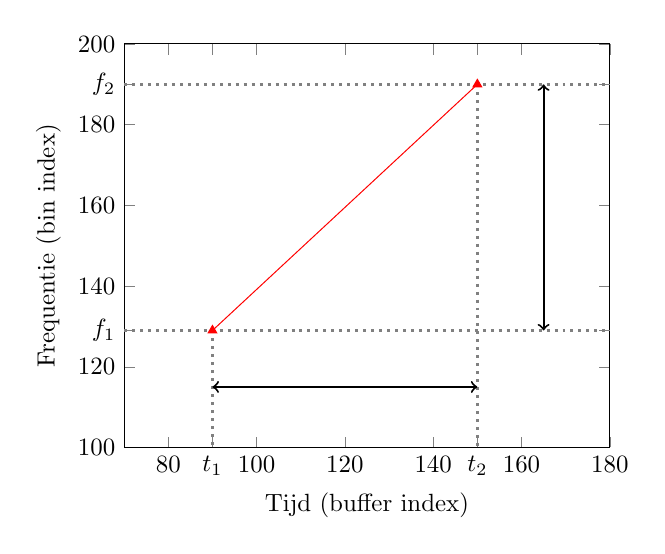
\begin{tikzpicture}[scale=0.9]
\begin{axis}[
	xlabel={Tijd (buffer index)},
	ylabel={Frequentie (bin index)},
	xmin=70,xmax=180,
	ymin=100,ymax=200,
	legend style={
  		cells={anchor=west},
  		legend pos=outer north east,
	},
	extra y ticks={129,190}, 
	extra y tick labels={$f_1$,$f_2$},
	extra x ticks={90,150}, 
	extra x tick labels={$t_1$,$t_2$},
]

  % plot the data from the file data.dat
  % smooth the curve and mark the data point with a dot
  \addplot[color=red,mark=triangle*] coordinates {
  	(90,129)
  	(150,190)
  };
  
  %f1
   \addplot[style= dotted,color=gray,very thick] coordinates{ (70,129)
   (180,129)};
   %f2
   \addplot[style= dotted,color=gray,very thick] coordinates{ (70,190)
   (180,190)};
   
    \node at (99,60) [] {\small$\Delta f$};
    \addplot[color=black,<->,thick] coordinates{ (165,129) (165,190)};
    
   \node at (50,18) [] {\small$\Delta t$};
   \addplot[style=dotted,color=gray,very thick] coordinates{ (90,129)
   (90,100)}; 
   \addplot[style=dotted,color=gray,very thick] coordinates{
   (150,190) (150,100)};
   \addplot[color=black,<->,thick] coordinates{ (90,115)
   (150,115)};
  
  \end{axis}
\end{tikzpicture}
	\end{center}
	\label{schematische-fingerprint}
\end{figure}

Bij het zoeken naar matches kan er gesteund worden op enkele typische eigenschappen van fingerprints: 

Twee overeenkomende fingerprints uit twee geluidsfragmenten zullen dezelfde frequenties  ($f1$ en $f2$) hebben. Bijgevolg is ook het verschil in frequentie ($\Delta f$) gelijk. 

De tijd van de spectrale pieken ($t1$ en $t2$) komen meestal niet overeen. Bij Shazam is het bijvoorbeeld geen vereiste om een opname te maken vanaf het begin van een liedje. Het moment van de opname mag volledig willekeurig worden gekozen. Bij het synchroniseren van streams wordt gezocht naar het verschil tussen de begintijden ($t1$ van elke fingerprint) van de overeenkomstige fingerprints van de audiofragmenten. Dit tijdverschil is wel gelijk bij elk paar overeenkomende fingerprints.

Hoewel de tijd ($t1$ en $t2$) van twee fingerprints meestal verschilt is dit niet het geval voor het verschil ervan ($\Delta t$). Bij twee overeenkomende fingerprints van twee audiofragmenten is het verschil in frequentie inherent gelijk.

Uit voorgaande eigenschappen kan geconcludeerd worden dat fingerprints uit twee audiofragmenten matchen wanneer $ f1 $, $ \Delta f $ en $ \Delta t $ gelijk zijn. Om deze parameters snel met elkaar kunnen te vergelijken wordt er een berekening uitgevoerd die deze parameters omzet in één enkel getal. Dit getal wordt de hash van de fingerprint genoemd. Samen met deze hash wordt ook $ t1 $ en een identificatie van het geluidsfragment bijgehouden.

Artikel \cite{six2014panako} geeft meer informatie over de omzetting van deze drie getallen tot een hash.

Een fingerprint kan bijgevolg gezien worden als verzameling gegevens met de volgende structuur: $ ( id; t1; hash(f1; \Delta f; \Delta t) ) $. Het zoeken naar fingerprints met overeenkomstige hashwaarden is mogelijk in $O(1)$ door gebruik te maken van een hashtabel. De precieze werking hiervan valt buiten de scope van deze scriptie.

Om te bepalen of twee audiofragmenten wel degelijk overeenkomen wordt er gezocht naar alle fingerprints met een overeenkomende hashwaarde. Van elk paar overeenkomende fingerprints wordt het verschil tussen $ t1 $ berekend. Dit verschil wordt de offset genoemd. Het vinden van een groot aantal matches met dezelfde offset wijst op een sterke gelijkenis tussen de audiofragmenten. De precieze waarde van ``een groot aantal'' wordt bepaald door een parameter van het algoritme.

\subsubsection{Bepalen van de latency}

Accoustic fingerprinting kan gebruikt worden om streams te synchroniseren door de ze eerst te bufferen. Wanneer een buffer volledig is opgevuld kan deze net zoals een kort audiofragment worden verwerkt door het algoritme. De latency tussen streams wordt bepaald door de offset die in vorig paragraaf werd beschreven: het verschil tussen de $ t1 $ waarden stelt namelijk de verschuiving tussen de geluidsfragmenten voor.

Figuur \ref{schematische-synchronisatie} toont schematisch alle stappen die moeten worden doorlopen om met behulp van accoustic fingerprinting audiostreams te synchroniseren.

\vspace{0.3cm}
\begin{figure}[h]
	\captionsetup{width=0.7\textwidth}
	\caption[Schema synchronisatie met fingerprinting]{Schematische voorstelling van synchronisatie met behulp van een accoustic fingerprinting systeem.}
	\advance\parskip0.5cm
	\begin{tikzpicture}[overlay]
\node at (-1,0) [minimum width=2cm] (A) {};

\node (rect) at (3,0) [draw,thin,minimum width=3cm,minimum height=1cm,align=center,font=\footnotesize] (B) {Feature \\[-0.7em] extractie};

\node (rect) at (8,0) [draw,thin,minimum width=3cm,minimum height=1cm,align=center,font=\footnotesize] (C) {Fingerprint \\[-0.7em] constructie};

\node (rect) at (13,-2) [draw,thin,minimum width=3cm,minimum height=1cm,align=center,font=\footnotesize] (G) {Andere \\[-0.7em] fingerprints};

\node (rect) at (13,0) [draw,thin,minimum width=3cm,minimum height=1cm,align=center,font=\footnotesize] (D) {Matchen en \\[-0.7em] bepalen latency};

\node at (17,0) [minimum width=2cm] (E) {};

\node at (0,-10) [minimum height=5cm] (F) {};

\draw [->] (A) -- (B) node [pos=0.4,above,align=center,font=\footnotesize] {Buffer};
\draw [->] (B) -- (C) node [pos=0.5,above,align=center,font=\footnotesize] {Features};
\draw [->] (C) -- (D) node [pos=0.5,above,align=center,font=\footnotesize] {Fingerprint};
\draw [->] (D) -- (E) node [pos=0.6,above,align=center,font=\footnotesize] {Latency};
\draw [->] (G) -- (D);

\end{tikzpicture}
	\advance\parskip1cm
	\label{schematische-synchronisatie}
\end{figure}
\vspace{2.5cm}

Een uitgebreidere beschrijving is te vinden in artikel \cite{Wang2003a}. De methode die in het artikel en deze scriptie besproken werd is beperkt tot het vergelijken van audiofragmenten die in tijd noch toonhoogte gewijzigd zijn. Aan het IPEM is een aangepaste methode ontwikkeld die dit wel toelaat \cite{six2014panako}.

\subsubsection{Nauwkeurigheid}

Zowel de snelheid waarmee wijzigingen van de latency bepaald kunnen worden als de nauwkeurigheid van de latency zelf hangt af van heel wat verschillende parameters van het algoritme.

De detectiesnelheid is vooral afhankelijk van de buffergrootte waarop het algoritme wordt uitgevoerd. Met deze instelling moet echter omzichtig worden omgegaan: een te kleine buffergrootte kan er toe leiden dat het algoritme niet meer in staat is om voldoende matches te vinden. Het kan helpen om andere parameters te wijzigen waardoor het vinden van een groot aantal matches gegarandeerd blijft. Deze parameters worden in sectie \ref{accoustic-fingerprinting-params} in detail besproken.

De nauwkeurigheid van de latency van het algoritme hangt af van de parameters van het FFT algoritme. Een nauwkeurigheid van 16 ms of 32 ms is standaard. De precieze werking van het FFT algoritme valt buiten de scope van deze scriptie.

\subsection{Kruiscovariantie}
\label{kruiscovariantie}

Deze methode bepaalt de gelijkenis tussen twee audiofragmenten en resulteert in één getal. Dit getal is een soort van score die aangeeft in welke mate twee signalen overeenkomen. De latency tussen twee audiofragmenten kan bepaald worden door deze berekening uit te voeren voor \textbf{elke mogelijke verschuiving}. De verschuiving waarbij het resulterend getal het hoogst is bepaalt de latency.

\subsubsection{Werking}

Stel twee audioblokken $ a $ en $ b $ bestaande uit een gelijk aantal samples ($n$). Deze audioblokken worden telkens cyclisch één sample verschoven tot wanneer de kruiscovariantie waarde ($ k $) voor elke mogelijke verschuiving berekend werd. De variabele $ i $ stelt de huidige verschuiving voor en gaat van 0 tot $ n $. De kruiscovariantie wordt berekend met formule:

\begin{equation}
	k = \sum_{j=0}^{n} a_{j} \cdot b_{(i+j)\ mod\ n}
\end{equation}

De waarde van $ i $ waarbij de kruiscovariantie het hoogst is stelt de latency voor tussen beide audioblokken in aantal samples. De latency in seconden kan bepaald worden door dit resultaat te delen door de samplefrequentie.

De methode kan de latency \textbf{tot op één sample nauwkeurig} bepalen. De maximaal bereikbare nauwkeurigheid hangt dus af van de samplefrequentie van de audioblokken. Bij een samplefrequentie van $8000 Hz$ is dit $ 1/8000 Hz = 0.125 ms $. Dit is ruim voldoende voor het huidige probleem.

Een nadeel aan deze methode is de performantie. Het berekenen van de beste kruiscovariantie van twee audioblokken bestaande uit $ n $ samples kan gebeuren in  $O(n^{2})$. Het is dus belangrijk om bij deze berekening de grootte van de audioblokken te beperken.

In artikel \cite{six2015multimodal} wordt deze techniek meer in detail besproken.

\subsubsection{Toepassing in realtime}

Het bufferen van de audiostreams maakt ook dit algoritme in realtime toepasbaar. In tegenstelling tot accoustic fingerprinting is het niet de bedoeling dat de berekeningen op de volledige buffer wordt uitgevoerd. Door de kwadratische tijdscomplexiteit zou het algoritme onnoemelijk veel rekenkracht vragen.\footnote{Voor het berekenen van de kruiscovariantie tussen twee buffers met $10s$ audio en een samplefrequentie van $8000hz$ zijn er asymptotisch $ 6.4 \cdot 10^9 $ berekeningen vereist.} Er moet dus een manier gevonden worden waarmee het mogelijk is om het aantal samples waarop het algoritme wordt uitgevoerd beperkt wordt.

\subsection{Toepasbaarheid}
\label{toepasbaarheid}

Het accoustic fingerprinting algoritme is zeer snel en robuust en kan gebruikt worden om gebufferde audiostreams te synchroniseren tot enkele tientallen milliseconden nauwkeurig (afhankelijk van de parameters van het FFT algoritme).

Het kruiscovariantie algoritme kan eveneens gebruikt worden om (gebufferde) audiostreams te synchroniseren. De grootste troef van dit algoritme is haar nauwkeurigheid: in de beste omstandigheden kan het algoritme resultaten bekomen tot op één sample nauwkeurig. Het bereiken van een dergelijke nauwkeurigheid is onmogelijk met eender welk ander besproken algoritme. De keerzijde is de performantie van het algoritme. Bij het synchroniseren van grote audioblokken kan dit problematisch zijn.

De kenmerken van deze algoritmen zijn complementair. De gemakkelijkste manier om een robuust, snel én nauwkeurig systeem op te bouwen is door het beste van de twee werelden te combineren. Het accoustic fingerprinting algoritme kan zorgen voor de synchronisatie tot op enkele tientallen milliseconden nauwkeurig. Dit resultaat laat toe dat we het kruiscovariantie algoritme kunnen uitvoeren op zeer korte stukjes audio (een honderdtal milliseconden volstaat).

\section{Bufferen van streams}
\label{streambuffers}

Aangezien de algoritmes een bepaalde hoeveelheid audio nodig hebben vooraleer ze kunnen worden uitgevoerd is het noodzakelijk om de streams eerst te bufferen. Dit proces moet herhaald worden aangezien er mogelijk samples gedropt worden of drift kan ontstaan. In dit deel zal worden uitgelegd hoe het bufferen precies in zijn werk gaat. Om verwarring met andere soorten buffers te vermijden zal dit type buffer verder in deze scriptie een \textit{streambuffer} genoemd worden.

\subsubsection{Buffergrootte}

De grootte van de buffer heeft invloed op de kwaliteit van de resultaten. Het spreekt voor zich dat het algoritme beter kan presteren wanneer er 10 seconden in plaats van 1 seconde audio geanalyseerd wordt. Een nadeel is echter dat het langer duurt vooraleer een wijzing van de latency gedetecteerd kan worden. 

\subsubsection{Naïeve implementatie}

Indien er buffers gebruikt worden die $ t $ aantal seconden audio kunnen bevatten, dan zal het bij een naïeve implementatie in het slechtste geval pas mogelijk zijn om een wijziging van de latency na $ \frac{3}{2} t $ seconden te detecteren. Dit is als volgt te verklaren: Een wijziging van de latency kan gedetecteerd worden wanneer meer dan de helft van de buffer gevuld is met audio met de nieuwe latency. Wanneer er samples gedropt worden net na het moment dat de buffer voor de helft gevuld is ($ \frac{1}{2} t $), dan zal het algoritme uitgevoerd op de huidige buffer de wijziging niet kunnen detecteren. De volgende buffer zal wel gevuld zijn audio met de nieuwe latency, het duurt echter nog een bijkomende $ t $ seconden vooraleer deze buffer gevuld is. De detectietijd bedraagt bijgevolg in het slechtste geval dus $ \frac{3}{2} t $ seconden.

De naïeve implementatie kan een wijziging van de latency in het beste geval na $ \frac{1}{2} t $ seconden detecteren. Wanneer er samples gedropt worden net voor het moment dat de buffer voor de helft gevuld is, dan kan het algoritme de nieuwe latency wel onmiddellijk detecteren.

\subsubsection{Sliding window}

Een meer doordachte manier van bufferen maakt gebruik van een \textit{sliding window}. In onderstaande beschrijving wordt gebruik gemaakt van een buffer met $ t $ seconden capaciteit en een stapgrootte van $ s $ seconden, hierbij geldt dat $ s \leq t $. 

Het verschil met de naïeve methode is dat de buffer niet pas na $ t $ seconden wordt opgeschoven. Door de buffer al na $ s $ seconden op te schuiven zal een wijziging van de latency sneller gedetecteerd kunnen worden; dit terwijl het algoritme toch nog steeds $ s $ seconden audio kan analyseren. In figuur \ref{slidingwindow} wordt grafisch weergegeven hoe de buffer precies verschoven wordt met $ t = 10 $ en $ s = 5 $.

\begin{figure}[h!]
	\captionsetup{width=0.7\textwidth}
	\caption[Schematische weergave van de buffer]{Schematische weergave van een \textit{sliding window} buffer over een audiostream.}
	\begin{center}
		\advance\parskip0.3cm
		\begin{tikzpicture}[scale=0.9]
\begin{axis}[
xlabel={Tijd (seconden)},
xmin=170,xmax=200,
ymin=0,ymax=1,
legend style={
	cells={anchor=west},
	legend pos=outer north east,
},
yticklabels={,,},
xticklabel style={grid=major},
extra x ticks={176,177,186,187},
extra x tick labels={,,,},
extra tick style={grid=major, grid style={dotted}},
hide y axis
]
\addplot[thick,black] graphics[xmin=140,ymin=0,xmax=200,ymax=1] {wave.png};

after end axis/.code={
	\draw[black,<->] (axis cs:175,0.1) -- (axis cs:185,0.1)	node [pos=0.5,above,font=\scriptsize] {buffer $i-1$};
	
	\draw[black,<->] (axis cs:176,0.2) -- (axis cs:186,0.2)	node [pos=0.5,above,font=\scriptsize] {buffer $i$};
	
	\draw[black,<->] (axis cs:177,0.3) -- (axis cs:187,0.3)	node [pos=0.5,above,font=\scriptsize] {buffer $i+1$};
}]

%\node at (50,18) [] {\small$\Delta t$};
%\addplot[style=dotted,color=gray,very thick] coordinates{ (90,129)
%	(90,100)}; 
%\addplot[style=dotted,color=gray,very thick] coordinates{
%	(150,190) (150,100)};
%\addplot[color=black,<->,thick] coordinates{ (90,115)
%	(150,115)};

\end{axis}

\end{tikzpicture}
	\end{center}
	\label{slidingwindow}
\end{figure}

Door de buffer al na $ s $ seconden op te schuiven wordt het slechtste geval sterk verbeterd. In het slechtste geval wordt een wijziging van de latency gedetecteerd na $ \frac{t}{2} + s $ seconden. Het beste geval blijft wel nog steeds $ \frac{t}{2} $ seconden.

Het verkleinen van de stapgrootte zorgt ervoor dat het algoritme per hoeveelheid audio frequenter moet worden uitgevoerd. Een te kleine stapgrootte heeft bijgevolg een negatieve invloed op de performantie.

\subsubsection{Voorbeeld}

Een praktisch voorbeeld zal bovenstaande beschrijving wat verduidelijken. In het voorbeeld worden twee audiostreams van 40 seconden geanalyseerd. Door het droppen van samples neemt de latency tussen de streams stapsgewijs toe. Figuur \ref{latency} toont in het zwart hoe de latency gedurende de verwerking evolueert. De opeenvolgende buffers van de twee besproken methode's worden in het rood aangeduid. 

\begin{figure}[h!]
	\captionsetup{width=0.7\textwidth}
	\caption[Voorbeeld buffering methodes]{Grafisch weergave van de methode's waarop gebufferd kan worden. De zwarte lijn stelt de huidige latency voor. In het rood worden de opeenvolgende buffers weergegeven.}
	\begin{center}
		\advance\parskip0.3cm
		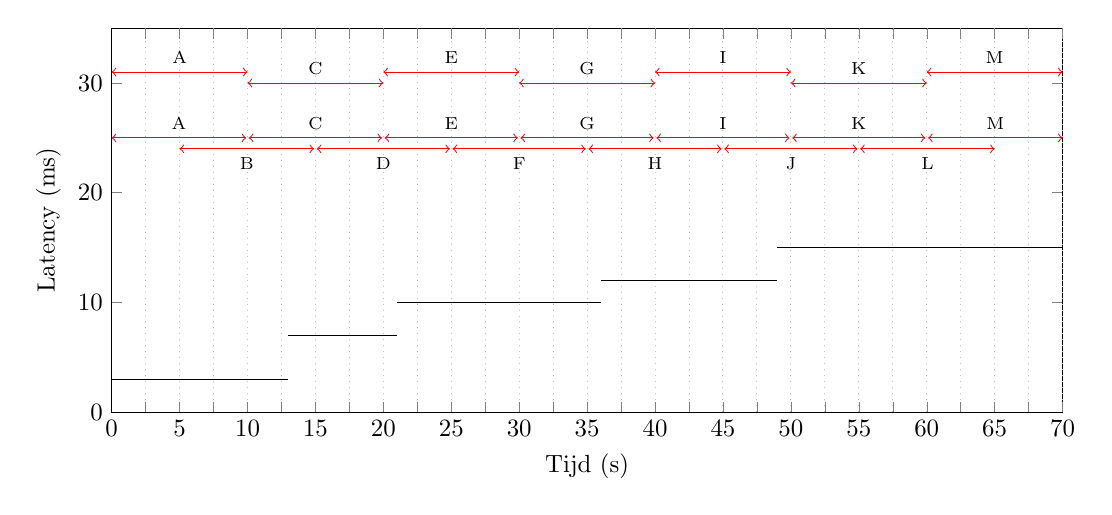
\begin{tikzpicture}[scale=0.9]
\begin{axis}[
xlabel={Tijd (s)},
ylabel={Latency (ms)},
xmin=0,xmax=70,
ymin=0,ymax=35,
legend style={
	cells={anchor=west},
	legend pos=outer north east,
},
extra x ticks ={2.5,5,7.5,...,70},
extra x tick labels={,,,},
extra x tick style={grid=major, grid style={dotted}},
width = 15cm,
height = 7cm
]



after end axis/.code={
	\draw (axis cs:0,3) -- (axis cs:13,3);
	\draw (axis cs:13,7) -- (axis cs:21,7);
	\draw (axis cs:21,10) -- (axis cs:36,10);
	\draw (axis cs:36,12) -- (axis cs:49,12);
	\draw (axis cs:49,15) -- (axis cs:70,15);
	
	\draw[red,<->] (axis cs:0,31) -- (axis cs:10,31)	node [pos=0.5,above,font=\scriptsize,color=black] {A};
	\draw[red,<->] (axis cs:10,30) -- (axis cs:20,30)	node [pos=0.5,above,font=\scriptsize,color=black] {C};
	\draw[red,<->] (axis cs:20,31) -- (axis cs:30,31)	node [pos=0.5,above,font=\scriptsize,color=black] {E};
	\draw[red,<->] (axis cs:30,30) -- (axis cs:40,30)	node [pos=0.5,above,font=\scriptsize,color=black] {G};
	\draw[red,<->] (axis cs:40,31) -- (axis cs:50,31)	node [pos=0.5,above,font=\scriptsize,color=black] {I};
	\draw[red,<->] (axis cs:50,30) -- (axis cs:60,30)	node [pos=0.5,above,font=\scriptsize,color=black] {K};
	\draw[red,<->] (axis cs:60,31) -- (axis cs:70,31)	node [pos=0.5,above,font=\scriptsize,color=black] {M};
	
	\draw[red,<->] (axis cs:0,25) -- (axis cs:9.9,25)	node [pos=0.5,above,font=\scriptsize,color=black] {A};
	\draw[red,<->] (axis cs:5,24) -- (axis cs:14.9,24)	node [pos=0.5,below,font=\scriptsize,color=black] {B};
	\draw[red,<->] (axis cs:10.1,25) -- (axis cs:19.9,25)	node [pos=0.5,above,font=\scriptsize,color=black] {C};
	\draw[red,<->] (axis cs:15.1,24) -- (axis cs:24.9,24)	node [pos=0.5,below,font=\scriptsize,color=black] {D};
	\draw[red,<->] (axis cs:20.1,25) -- (axis cs:29.9,25)	node [pos=0.5,above,font=\scriptsize,color=black] {E};
	\draw[red,<->] (axis cs:25.1,24) -- (axis cs:34.9,24)	node [pos=0.5,below,font=\scriptsize,color=black] {F};
	\draw[red,<->] (axis cs:30.1,25) -- (axis cs:39.9,25)	node [pos=0.5,above,font=\scriptsize,color=black] {G};
	\draw[red,<->] (axis cs:35.1,24) -- (axis cs:44.9,24)	node [pos=0.5,below,font=\scriptsize,color=black] {H};
	\draw[red,<->] (axis cs:40.1,25) -- (axis cs:49.9,25)	node [pos=0.5,above,font=\scriptsize,color=black] {I};
	\draw[red,<->] (axis cs:45.1,24) -- (axis cs:54.9,24)	node [pos=0.5,below,font=\scriptsize,color=black] {J};
	\draw[red,<->] (axis cs:50.1,25) -- (axis cs:59.9,25)	node [pos=0.5,above,font=\scriptsize,color=black] {K};
	\draw[red,<->] (axis cs:55.1,24) -- (axis cs:65,24)	node [pos=0.5,below,font=\scriptsize,color=black] {L};
	\draw[red,<->] (axis cs:60.1,25) -- (axis cs:70,25)	node [pos=0.5,above,font=\scriptsize,color=black] {M};
	
%	\draw[black,<->] (axis cs:10,0.2) -- (axis cs:20,0.2)	node [pos=0.5,above,font=\scriptsize] {buffer $i$};
	
%	\draw[black,<->] (axis cs:20,0.3) -- (axis cs:30,0.3)	node [pos=0.5,above,font=\scriptsize] {buffer $i+1$};
}]

\end{axis}

\end{tikzpicture}
	\end{center}
	\label{latency}
\end{figure}

De initiële latency van 3 milliseconden wordt zowel met de naïeve methode als met het sliding window gedetecteerd na de analyse van de allereerste buffer (A of R) 10 seconden na aanvang van de analyse. De eerste verhoging tot 7 milliseconden vindt te laat plaats om gedetecteerd te kunnen worden door de eerste buffer van beide methodes. Bij deze verhoging van de latency wordt het verschil tussen beide methodes zichtbaar: bij  de sliding window methode vindt de detectie 6 seconden na de wijziging plaats. Bij de naïeve methode moet er echter gewacht worden tot wanneer buffer B is volgelopen 12 seconden na de wijziging. De tweede verhoging naar 10 seconden wordt zowel door de naïeve methode als door de sliding window methode gedetecteerd na 8 seconden (buffer C of W). De laatste wijziging naar 12 seconden kan door de naïeve methode pas gedetecteerd worden na 14 seconden (de buffer is niet meer zichtbaar op de grafiek). De sliding window methode zal deze wijziging na 6 seconden detecteren.

\subsubsection{Conclusie}

De detectiesnelheid van een latencywijziging hangt af van twee parameters: de bufferlengte ($t$) en de staplengte ($s$). Het beste geval ($ T_b $) heeft volgende ondergrens:
\begin{equation}
T_b = \frac{t}{2}
\end{equation}

Bij het slechtste geval ($ T_s $) moet ook rekening gehouden worden met de stapgrootte. De bovengrens wordt als volgt bepaalt:
\begin{equation}
T_s = \frac{t}{2} + s
\end{equation}

Bij het toepassen van deze formules op het voorbeeld uit het vorige paragraaf kan er worden vastgesteld dat in het beste geval een latencywijziging gedetecteerd kan worden na 5 seconden. In het slechtste geval wordt een dergelijke wijziging bij de naïeve methode ($t = s = 10 $) pas gedetecteerd na 15 seconden. Bij de sliding window methode ($t = 10, s = 4 $) is deze wachttijd echter begrensd tot maximaal 9 seconden.

%Evaluatiecriteria
\chapter{Implementatie}

\section{Technologieën en software}

\subsection{Java 7}

Er zijn verschillende redenen waarom er gekozen is om de synchronisatie bibliotheek in Java te implementeren. De belangrijkste reden is dat de bestaande audio bibliotheken (Panako en TarsosDSP) van het IPEM ook ontwikkeld zijn in Java. Deze kunnen enkel aangeroepen worden via andere Java applicaties.

Het is ook de bedoeling is om de gebruikersinterface te ontwikkelen met behulp van Max/MSP modules. Het ontwikkelen van dergelijke modules is mogelijk in twee programmeertalen: C en Java. De eenvoud en hoge graad van abstractie gaf de doorslag om hierbij Java te gebruiken. De voordelen die C biedt op vlak van snelheid wegen (in deze toepassing) hier niet tegenop.

Hoewel de laatste versie van Max/MSP (7) het toelaat om Java 8 te gebruiken wordt deze versie in dit project om compatibiliteitsredenen vermeden. 

\subsection{JUnit}
JUnit is een unit testing framework voor Java. JUnit heeft in dit onderzoek een belangrijke rol gespeeld bij het bepalen van de optimale parameters van de verschillende algoritmen. JUnit maakte het mogelijk om de algoritmes herhaald maar met verschillende parameters op een dataset los te laten. JUnit liet toe om in één oogopslag te zien hoe het algoritme heeft gepresteerd.

\subsection{TarsosDSP}
\label{tarsos}

TarsosDSP is een Java bibliotheek voor realtime audio analyse en verwerking ontwikkeld aan het IPEM. De bibliotheek bevat een groot aantal algoritmes voor audioverwerking en kan nog verder worden uitgebreid. Deze bibliotheek wordt beschreven in artikel \cite{six2014tarsosdsp}. 

%Volgende paragraaf eventueel verplaatsen naar 3.5.1, ben er nog niet helemaal uit.
TarsosDSP is voornamelijk gebouwd rond het concept \textit{processing pipeline}. Dit is een abstractie van een audiostream die via programmacode verwerkt kan worden. Een processing pipeline wordt voorgesteld als instantie van de klasse \texttt{AudioDispatcher}. Een \texttt{AudioDispatcher} kan aangemaakt worden van een audiobestand, een array van floating-point getallen of een microfoon en kan bewerkt of verwerkt worden met behulp van één of meerdere \texttt{AudioProcessors}. Objecten van klassen die de interface \texttt{AudioProcessor} implementeren kunnen aan de processing pipeline worden toegevoegd. In de implementatie van de \texttt{process} methode kan de audiostream op een bepaalde manier verwerkt, geanalyseerd of gewijzigd worden.

TarsosDSP bevat verder nog een groot aantal klassen met allerhande tools en audioverwerkings algoritmen. Een greep uit de features van TarsosDSP:
\begin{itemize}[noitemsep]
	\item Toevoegen van geluidseffecten (delay, flanger,...)
	\item Toevoegen van filters (low-pass, high-pass, band-pass,...)
	\item Conversie tussen verschillende formaten
	\item Toonhoogte detectie
	\item Wijzigen van de samplefrequentie
\end{itemize}

\subsection{Panako}

Panako is net zoals TarsosDSP een Java bibliotheek (door de zelfde auteur) ontwikkeld aan het IPEM. Panako bevat een arsenaal aan algoritmen voor het matchen of synchroniseren van audiofragmenten of audiostreams.  Deze bibliotheek wordt uitgebreid beschreven in artikel \cite{six2014panako}.

Dit onderzoek gebruikt Panako's open-source implementatie van het accoustic fingerprinting algoritme dat beschreven is in artikel \cite{Wang2003a}. Panako bevat ook een uitbreiding van het algoritme dat overweg kan met audio waarbij de toonhoogte verhoogd of verlaagd is, of waarbij de audio sneller of trager is afgespeeld.

Buiten het algoritme bevat de bibliotheek ook verschillende toepassingen die hiervan gebruik maken. Zo is het mogelijk om de fingerprints van een geluidsfragment te bekijken, matches tussen verschillende geluidsfragmenten te visualiseren, en grafisch te experimenteren met de verschillende parameters. Figuur \ref{fingerprint_visualiser} toont een screenshot van deze toepassing.

\begin{figure}[!h]
	\captionsetup{width=0.8\textwidth}
	\caption[Gebruikersinterface van Audacity]{De gebruikersinterface van Panako's NFFT Fingerprint Visualiser. Onderaan kunnen de parameters van het algoritme met behulp van sliders gewijzigd worden.}
	\centering
	\advance\parskip0.3cm
	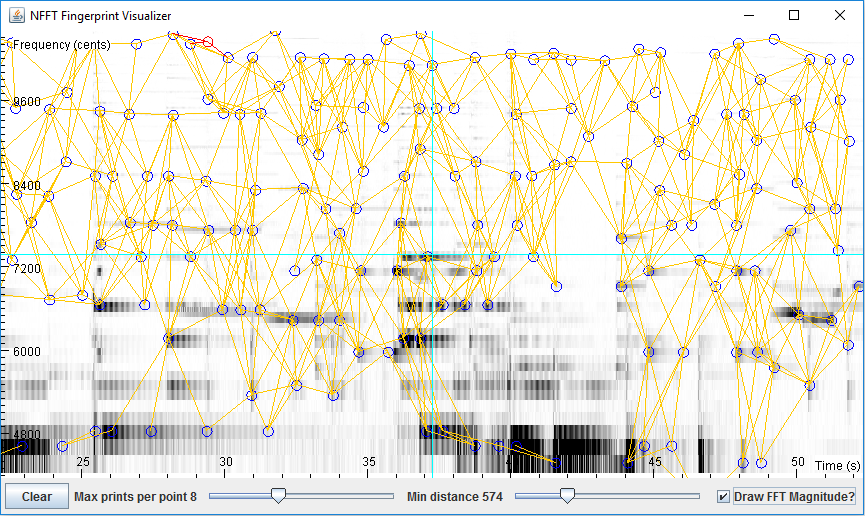
\includegraphics[width=0.8\textwidth]{fingerprint_visualiser.png}
	\label{fingerprint_visualiser}
\end{figure}

Er is ook een applicatie beschikbaar om verschillende geluidsfragmenten te synchroniseren. Deze applicatie gebruikt naast het accoustic fingerprinting algoritme ook het kruiscovariantie algoritme. 

Na het bepalen van de latency tussen de verschillende audiofragmenten kan de applicatie een shell script genereren dat met behulp van \textit{FFmpeg} stukjes van de geluidsbestanden wegknipt of er stilte aan toevoegt. Het resultaat is dat na het uitvoeren van het script de geluidsbestanden gesynchroniseerd zijn.

\subsection{FFmpeg}

FFmpeg is een command-line multimedia framework dat gebruikt wordt voor encoderen, decoderen, multiplexen, demultiplexen, streamen en afspelen van audio en video. \cite{kollarconfiguration}

In dit onderzoek wordt FFmpeg voornamelijk gebruikt in scripts bij het geautomatiseerd genereren van testdata.

\subsection{SoX}

SoX is net zoals FFmeg een command-line tool voor audioverwerking. Buiten de mogelijkheid om audiobestanden te converteren laat SoX ook minder triviale operaties toe. Zo is het onder meer mogelijk om het volume aan te passen, effecten toe te voegen, de bestanden bij te knippen of gegenereerde geluiden in een audiobestand te mixen.
\cite{barras2012sox}

In dit onderzoek wordt SoX gebruikt in scripts bij het manipuleren van de testdata.

\subsection{Sonic Visualiser}

Sonic Visualiser is een gebruiksvriendelijke desktopapplicatie voor de analyse, visualisatie van audiobestanden. Sonic Visualiser laat toe om audiobestanden vanuit verschillende perspectieven te analyseren, zo kan zowel de waveform als het spectrogram van een audiobestand gevisualiseerd worden. Sonic Visualiser is uitbreidbaar met plug-ins in het Vamp formaat. \cite{cannam2010sonic}

\begin{figure}[!h]
	\captionsetup{width=0.8\textwidth}
	\caption[Gebruikersinterface van Sonic Visualiser]{De gebruikersinterface van Sonic Visualiser}
	\advance\parskip0.3cm
	\centering
	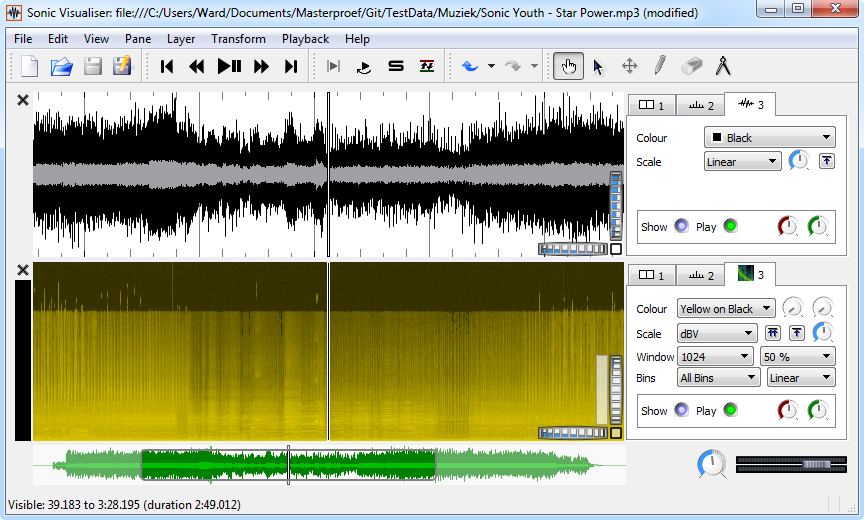
\includegraphics[width=0.8\textwidth]{sonicvisualiser.png}
\end{figure}

Sonic Visualiser werd in dit onderzoek vooral gebruikt om handmatig de latency tussen verschillende audiofragmenten te bepalen. Ook heeft de applicatie dienst gedaan als educatieve tool om verschillende audioverwerkingsalgoritmen visueel voor te stellen.
\vspace{0.5cm}

\subsection{Audacity}

Audacity is een open-source desktopapplicatie voor het bewerken, opnemen en converteren van audio. Met Audacity is het ook mogelijk om tal van effecten en filters aan audio toe te voegen.\cite{audacity2016} 

Figuur \ref{screenshot-audacity} toont de gebruikersinterface van dit programma.

\begin{figure}[!h]
	\captionsetup{width=0.8\textwidth}
	\caption[Gebruikersinterface van Audacity]{De gebruikersinterface van Audacity}
	\centering
	\advance\parskip0.3cm
	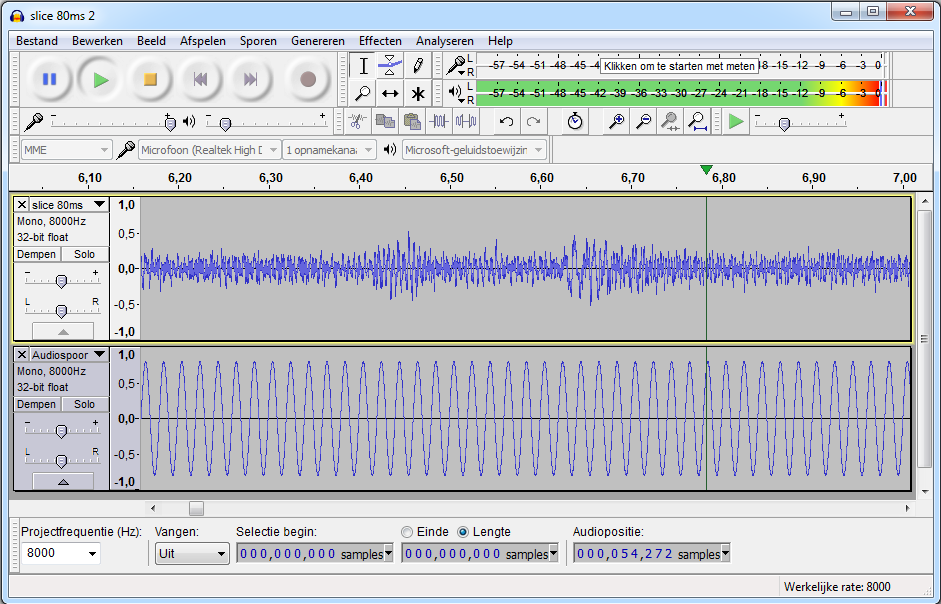
\includegraphics[width=0.8\textwidth]{audacity.png}
	\label{screenshot-audacity}
\end{figure}

Alle opnames en handmatige bewerkingen op audiobestanden in dit onderzoek zijn uitgevoerd met behulp van Audacity. 

\subsection{Max/MSP}

Max/MSP is een visuele programmeertaal voor muziek en multimedia. Het is een systeem waarbij modules met elkaar verbonden kunnen worden om zo complexere systemen op te bouwen. Max/MSP beschikt ook over een API waarmee in Java of C nieuwe modules ontwikkeld kunnen worden. \cite{cycling2016}

\begin{figure}[!h]
	\captionsetup{width=0.8\textwidth}
	\caption[Gebruikersinterface van Max/MSP]{De gebruikersinterface van Max/MSP: een \textit{patch panel} met daarop enkele modules die samen een complexere toepassing vormen.}
	\centering
	\advance\parskip0.3cm
	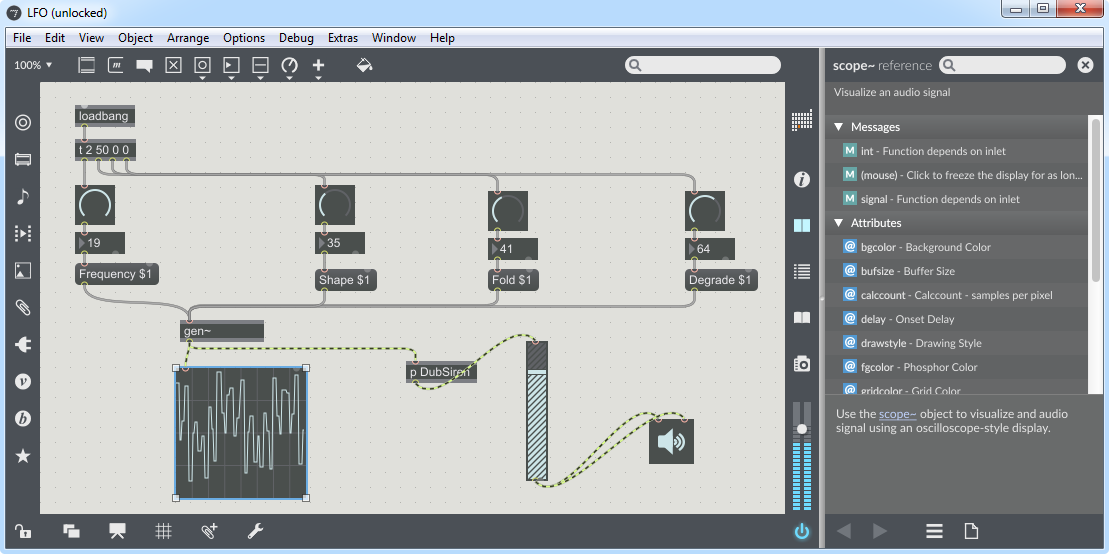
\includegraphics[width=0.8\textwidth]{maxmsp.png}
	\label{screenshot-max}
\end{figure}

Met Max/MSP is het mogelijk om realtime audio te  verwerken, daarom zal deze toepassing gebruikt worden voor het ontwikkelen van de gebruikersinterface. 

Figuur \ref{screenshot-max} toont hoe een eenvoudige Max/MSP patch er grafisch uitziet.

\subsection{Teensy}

De Teensy is een kleine microcontroller die via USB geprogrammeerd kan worden. De Teensy is compatibel met de Arduino software en is hierdoor zeer gebruiksvriendelijk. \cite{teensy2016}

De sensoren die gebruikt worden bij de experimenten van het IPEM zijn meestal aangesloten op Teensy microcontrollers.

\begin{figure}[!h]
	\captionsetup{width=0.7\textwidth}
	\caption[Teensy microcontroller]{De Teensy microcontroller verbonden met een infraroodsensor en microfoon op een breadboard.}
	\centering
	\advance\parskip0.3cm
	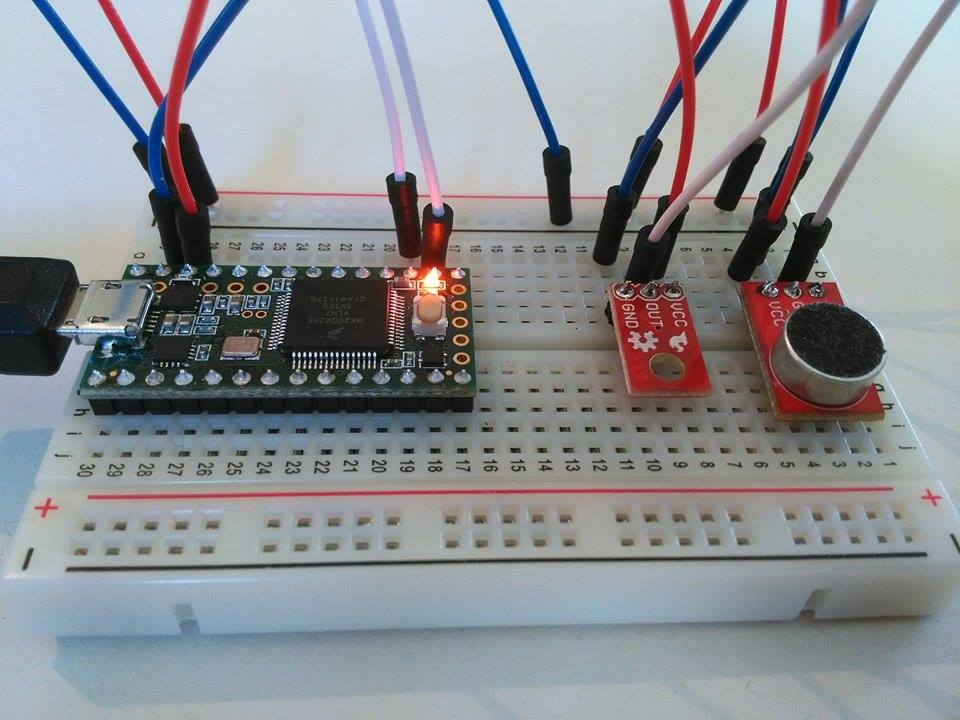
\includegraphics[width=0.4\textwidth]{teensy.jpg}
	\label{teensy-pic}
\end{figure}

In hoofdstuk \ref{evaluatie} worden de testen die met de Teensy microcontroller zijn uitgevoerd meer in detail besproken. Figuur \ref{teensy-pic} toont een typische testopstelling waarbij twee sensoren zijn aangesloten op de microcontroller.

\section{Accoustic fingerprinting}

De Panako softwarebibliotheek bevat een implementatie van het accoustic fingerprinting algoritme. Om wijzigingen mogelijk te maken hebben is de code van het algoritme overgenomen in het project van dit onderzoek. De aangepaste code blijft wel nog steeds afhankelijk van enkele klassen uit het Panako project. 

\subsection{Optimalisaties}

Aan dit algoritme is één vereenvoudiging aangebracht. Het originele algoritme bevatte namelijk de mogelijkheid om alle offsets boven een bepaalde drempelwaarde te verwerken. Deze feature laat toe dat er meerdere matches kunnen gevonden worden binnen één uitvoering van het algoritme. Om dit te ondersteunen moeten alle matches echter wel één voor één worden vergeleken met de drempelwaarde. Omdat deze toepassing enkel de beste offsetwaarde nodig heeft is dit overbodig. De beste offset en bijhorende fingerprints wordt apart bijgehouden. De naverwerking wordt hierdoor vermeden.

\subsection{Parameters en hun invloed op het algoritme}
\label{accoustic-fingerprinting-params}

De werking van dit algoritme is afhankelijk van een aantal parameters die een grote invloed kunnen hebben op de performantie en de nauwkeurigheid van het uiteindelijke resultaat. Daarom is het van belang om voor het uitvoeren van het algoritme de waarde van deze parameters te controleren. De optimale waarde van elke parameter is afhankelijk van verschillende factoren die van situatie tot situatie kunnen verschillen:

\begin{itemize}[noitemsep]
\item de vereiste nauwkeurigheid van het algoritme;
\item de vereiste performantie van het algoritme;
\item de mate waarin er omgevingsgeluid aanwezig is;
\item de opnamekwaliteit van het omgevingsgeluid.
\end{itemize}

De meeste parameters worden bijgehouden in een configuratiebestand waardoor ze ook na compilatie wijzigbaar zijn. Dit zijn de belangrijkste parameters uit het configuratiebestand die invloed hebben op het algoritme:

\begin{description}
\item\texttt{SAMPLE\_RATE} \hfill \\
Deze parameter bepaalt de standaard samplefrequentie die gebruikt wordt tijdens het synchronisatieproces. Het verhogen van deze parameter zorgt voor een tragere verwerking maar een betere nauwkeurigheid. Afhankelijk van op welke manier de synchronisatie wordt opgestart (via Max of met een \texttt{AudioDispatcher}) worden de binnenkomende streams geresamplet of wordt al een correcte samplefrequentie verondersteld.

\item\texttt{NFFT\_BUFFER\_SIZE}\footnote{De letter N in NFFT heeft geen noemenswaardige betekenis. De naam is overgenomen van de gelijknamige parameter uit de Panako bibliotheek.} \hfill \\
Dit is de grootte van de verschuivende buffer die gebruikt wordt in het FFT algoritme. Deze parameter is cruciaal aangezien de frequentiesterktes op een bepaalde plaats op de tijd\-as worden berekend per buffer. Deze parameter wordt uitgedrukt in aantal samples.
\item\texttt{NFFT\_STEP\_SIZE} \hfill \\
Dit is het aantal samples elke verschuiving in het FFT algoritme. De stepsize beïnvloedt rechtstreeks de nauwkeurigheid van het accoustic fingerprinting algoritme. Wanneer deze parameter is ingesteld op 128 samples en een samplefrequentie van 8000hz dan is de maximale nauwkeurigheid $128/8000Hz = 0.016s = 16ms$.
\item\texttt{MIN\_ALIGNED\_MATCHES} \hfill \\
Een match tussen twee audiofragmenten wordt pas als geldig beschouwd wanneer er een bepaald aantal fingerprint matches met dezelfde offset gevonden zijn. Dit aantal wordt ingesteld met deze parameter.
\item\texttt{NFFT\_MAX\_FINGERPRINTS\_PER\_EVENT\_POINT} \hfill \\
Deze parameter bepaalt het maximum aantal fingerprints waaraan een event point (een punt op het spectrogram) kan deelnemen. Hoe hoger dit maximum hoe vlugger er matches kunnen gevonden worden. Bij een hoge waarde moeten meer berekeningen worden uitgevoerd, dit heeft invloed op de performantie.
\item\texttt{NFFT\_EVENT\_POINT\_MIN\_DISTANCE} \hfill \\
Dit is de minimale afstand tussen twee event points op het spectrogram die samen een fingerprint kunnen vormen. 

\end{description}

Verder maakt het algoritme nog gebruik van twee hardgecodeerde parameters die niet instelbaar zijn via het configuratiebestand: \texttt{MIN\_FREQUENCY} en \texttt{MAX\_FREQUENCY}. Deze parameters bepalen binnen welke frequentiebereik er naar fingerprints gezocht worden. De waarden waarop deze ingesteld staan bevinden zich op de rand van de frequenties die door muziek of stemgeluid geproduceerd worden.

\subsection{Optimale instellingen}
\label{optimal-accoustic-fingerprinting}

Het bepalen van de optimale waarden voor de parameters is geen exacte wetenschap maar eerder een probleem dat proefondervindelijk moet worden aangepakt.

Bij het accoustic fingerprinting algoritme is er een groot verschil tussen de meest ``elegante'' parameterwaarden en de in de praktisch presterende waarden. Dit verschil zal duidelijk worden in volgende opsomming waarin elke parameter zal worden besproken.


\begin{description}
	\item\texttt{SAMPLE\_RATE} \hfill \\
	Bij deze parameter is het van belang om een goede balans te vinden zodat de geluidskwaliteit aanvaardbaar blijft zonder een hypotheek te plaatsen op de performantie van het algoritme. De praktijk heeft uitgewezen dat bij een samplefrequentie van $ 8000Hz $ het algoritme goed presteert. Deze waarde wordt bevestigd in artikel \cite{six2015multimodal}.
	\item\texttt{NFFT\_BUFFER\_SIZE} en \texttt{NFFT\_STEP\_SIZE} \hfill \\
	De ingesteld waarden van de samplefrequentie, buffergrootte en stapgrootte zijn afhankelijk van elkaar. Om een goede werking van het FFT algoritme te garanderen bij een samplefrequentie van $ 8000Hz $ worden de buffergrootte en stapgrootte respectievelijk ingesteld op 512 en 128 (of 256) samples. Deze waarden worden eveneens vermeld in artikel \cite{six2015multimodal}.
	\item\texttt{MIN\_ALIGNED\_MATCHES} \hfill \\
	In een toepassing zoals het detecteren van liedjes ten opzichte van een database is het secuur instellen van deze parameter erg belangrijk. Deze parameter heeft namelijk een grote invloed op het voorkomen van \textit{false positives} of \textit{false negatives}. 
	
	Bij het synchroniseren van streams is de situatie echter helemaal anders. Het binnenkrijgen van een false positive (=foute latency) is veel minder erg dan het helemaal niet binnenkrijgen van (mogelijk correcte) resultaten. Aangezien het algoritme per buffer enkel het beste resultaat teruggeeft is de kans dat bij geluidsfragmenten van behoorlijke kwaliteit eenzelfde foute latency meer voorkomt dan de correcte latency zéér klein.
	
	Bij geluidsfragmenten van mindere kwaliteit kan het gebeuren dat er toch foute resultaten door de mazen van het net glippen. Om dit te vermijden is het mogelijk om nog een extra filtering toe te passen. In deze extra stap worden eventuele uitschieters geëlimineerd.
	
	Bovenstaande argumenten stellen duidelijk dat het beter is om deze parameter een lage waarde te geven. In deze toepassing is gekozen voor de waarde 2 in plaats van het absolute minimum 1: hierdoor wordt pure willekeur bij het matchen van audiofragmenten van extreem slechte kwaliteit vermeden. Dit is laag in vergelijking met Panako waar 7 de standaard waarde is van deze parameter.
	
	\item\texttt{NFFT\_MAX\_FINGERPRINTS\_PER\_EVENT\_POINT} \hfill \\
	In Panako is het standaard dat een event point uitmaakt van maximaal 2 fingerprints. Het hanteren van deze waarde leidt ertoe dat het matchen van audiofragmenten van behoorlijke kwaliteit zeer snel kan worden uitgevoerd. 
	
	In deze toepassing is het aantal te vergelijken audiofragmenten meestal erg beperkt. Ook is de kwaliteit van deze fragmenten vaak van ondermaats (bv. de opnames op microcontrollers). Daarom is het in dit geval een goed idee om de waarde van deze parameter zéér hoog in te stellen. Hierdoor verhoogt de kans sterk dat er bij zeer slechte audiofragmenten toch enkele overeenkomende fingerprints gevonden worden. Testen hebben uitgewezen dat de negatieve invloed op de performantie beperkt blijft en dat de resultaten sterk verbeteren. 
	
	Bij het zoeken naar matches tussen geluidsopnames opgenomen op microcontrollers heeft de praktijk uitgewezen dat het toelaten van maximaal 50 fingerprints per event point degelijke resultaten oplevert.
	%TODO: refereren naar testresultaen
	
	\item\texttt{NFFT\_EVENT\_POINT\_MIN\_DISTANCE} \hfill \\
	In tegenstelling tot vorige parameter zorgt het verhogen van deze waarde ervoor dat er minder fingerprints worden gecreëerd. De argumenten die bij vorige parameter zijn aangehaald gelden bijgevolg in omgekeerde zin ook voor deze parameter. Hoewel de Panako standaard 600 is leveren waardes rond het getal 20 in deze toepassing de beste resultaten zonder de performantie sterk te beperken.
	
	
\end{description}


\section{Kruiscovariantie}

De Panako bibliotheek bevatte bij aanvang van dit onderzoek al een implementatie van het kruiscovariantie algoritme. In tegenstelling tot het accoustic fingerprinting algoritme was het echter minder grondig afgewerkt. Om degelijke resultaten te garanderen was het noodzakelijk om enkele anomalieën in de geleverde resultaten te analyseren en de oorzaak hiervan op te lossen.

Net zoals het accoustic fingerprinting algoritme is de code overgenomen in het project van dit onderzoek. De code is niet meer afhankelijk van de Panako bibliotheek.

\subsection{Integratie met accoustic fingerprinting}
\label{integratie-accoustic-fingerprinting}

In sectie \ref{toepasbaarheid} is er geschreven dat de latency zeer nauwkeurig kan bepaald worden door het berekenen van de kruiscovariantie. Vanwege de performantie is het wel noodzakelijk om eerst de ruwe latency met accoustic fingerprinting te bepalen. Hoe deze algoritmes geïntegreerd worden zal hier worden besproken. 

Onderstel twee geluidsopnames: de tweede opname heeft een vertraging van 90 ms ten opzichte van de eerste referentieopname. Het uitvoeren van het accoustic fingerprinting algoritme met standaard parameters (tot op $ 32 ms $ nauwkeurig) kan twee resultaten opleveren: $ 64 ms $ of $ 96 ms $. Bij het eerste resultaat wordt de werkelijke latency onderschat. De tweede latency overschat deze waarde. Na het berekenen van de kruiscovariantie kan bepaald worden of er zich een onderschatting of overschatting heeft voorgedaan, dit is van belang om het resultaat correct te verfijnen. Figuur \ref{crosscovariance1} toont de mogelijke resultaten van het algoritme.

Als de ruw bepaalde latency positief is wordt deze waarde van het tweede fragment weggeknipt. Na deze stap is de latency van het resterende audiofragment zeker minder dan de minimale nauwkeurigheid van het accoustic fingerprinting algoritme. 

\begin{figure}[h!]
	\captionsetup{width=0.7\textwidth}
	\caption[Kruiscovariantie audiofragmenten]{Twee audiofragmenten: het tweede audiofragment heeft een latency van 90 milliseconden ten opzichte van het eerste.}
	\begin{center}
		\advance\parskip0.3cm
		\begin{tikzpicture}[scale=1]
\begin{axis}[
xlabel={Tijd (milliseconden)},
xmin=0,xmax=500,
ymin=0,ymax=1,
legend style={
	cells={anchor=west},
	legend pos=outer north east,
},
yticklabels={,,},
xticklabel style={grid=major},
extra x ticks ={64,90,96},
extra x tick labels={,,,},
extra tick style={grid=major, grid style={dotted}},
hide y axis
]

\addplot[thick,black] graphics[xmin=0,ymin=0.5,xmax=500,ymax=0.8] {reference.png};

\addplot[thick,black] graphics[xmin=0,ymin=0.0,xmax=500,ymax=0.3] {other.png};


after end axis/.code={

	
	\draw[black,<->] (axis cs:0,0.42) -- (axis cs:96,0.42)	node [pos=0.5,above,font=\scriptsize] {$96ms$};
	
	\draw[black,<->] (axis cs:0,0.32) -- (axis cs:90,0.32)	node [pos=0.5,above,font=\scriptsize] {$90ms$};
	
	\draw[black,<->] (axis cs:0,0.22) -- (axis cs:64,0.22)	node [pos=0.5,above,font=\scriptsize] {$64ms$};
}]

\node at (axis cs:250,0.82) [] {Referentie};
\node at (axis cs:250,0.35) [] {Andere};

\end{axis}

\end{tikzpicture}
	\end{center}
	\label{crosscovariance1}
\end{figure}


Vervolgens worden een aantal samples van elk audiofragment gekopieerd naar een buffer. De latency tussen deze twee buffers wordt berekend met het kruiscovariantie algoritme (beschreven in sectie \ref{kruiscovariantie}). Figuur \ref{crosscovariance2} toont de buffers waarop het algoritme kan worden uitgevoerd bij een buffergrootte van 512 samples en samplefrequentie van $ 8000Hz $.

\begin{figure}[h!]
	\captionsetup{width=0.7\textwidth}
	\caption[Kruiscovariantie buffers]{Kruiscovariantie buffers na het wegknippen van de $ 96 ms $ latency bepaald door het accoustic fingerprinting algoritme. Hier heeft de referentie audio $ 6 ms $ latency ten opzichte van het andere audiofragment.   }
	\begin{center}
		\advance\parskip0.3cm
		\begin{tikzpicture}[scale=1]
\begin{axis}[
xlabel={Tijd (milliseconden)},
xmin=0,xmax=64,
ymin=0,ymax=1,
legend style={
	cells={anchor=west},
	legend pos=outer north east,
},
yticklabels={,,},
xticklabel style={grid=major},
%extra x ticks ={64,90,96},
extra x tick labels={,,,},
extra tick style={grid=major, grid style={dotted}},
hide y axis,
width = 15cm,
height = 7cm
]

\addplot[thick,black] graphics[xmin=0,ymin=0.6,xmax=64,ymax=0.9] {refcut.png};

\addplot[thick,black] graphics[xmin=0,ymin=0.1,xmax=64,ymax=0.4] {othercut.png};


after end axis/.code={
	\draw[black,<->] (axis cs:0,0.85) -- (axis cs:6,0.85)	node [pos=0.5,above,font=\scriptsize] {$6ms$};
}]

\node at (axis cs:32,0.85) [] {Referentie};
\node at (axis cs:32,0.37) [] {Andere};

\end{axis}

\end{tikzpicture}
	\end{center}
	\label{crosscovariance2}
\end{figure}

Wanneer het accoustic fingerprinting algoritme de werkelijke latency heeft onderschat wordt de verfijnde latency bekomen door de ruwe latency en het resultaat van het kruiscovariantie algoritme op te tellen. Bij een overschatting is dit niet het geval.

Aangezien het kruiscovariantie algoritme de latency zoekt van de ``andere'' buffer ten opzichte van de referentiebuffer zal het resultaat niet $6 ms$ maar $ 58 ms $ zijn. Dit komt doordat het algoritme de ``andere'' buffer cyclisch (maar in de verkeerde zin) verschuift.

Om in een dergelijke situatie de verfijnde latency te berekenen moet men van de som van de resultaten ($96 ms + 58 ms$) nog de lengte van de gebruikte buffer ($ 64ms $) aftrekken. De verfijnde latency is dus $ 154 ms - 64 ms = 90 ms $.

%Eventueel nog schrijven hoe bepaald wordt of het resultaat onderschat of overschat is.

\subsection{Optimalisaties}

\subsubsection{Bugfixes}

In de originele versie van het algoritme werd er geen rekening gehouden met het feit dat het accoustic fingerprinting algoritme het de werkelijke latency kan overschatten of onderschatten. De latency bepaalt door het kruiscovariantie algoritme werd telkens opgeteld bij de ruwe latency bepaald door het accoustic fingerprinting algoritme. In 50\% van de gevallen leidde dit probleem tot foutieve resultaten.

\subsubsection{Meerdere malen uitvoeren van het algoritme}
\label{crosscovariance-repeated}

In tegenstelling tot accoustic fingerprinting is het bepalen van de latency met kruiscovariantie veel meer foutgevoelig. Bij opnames van slechte kwaliteit worden vaak foute resultaten teruggegeven. 

Hoewel bij accoustic fingerprinting mogelijk storende factoren (een zoemende toon, geruis,...) zichtbaar zijn in het spectrogram zullen er naar alle waarschijnlijkheid nog steeds voldoende fingerprints gegenereerd worden op basis van geluiden die wel in beide opnames voorkomen. 

\begin{figure}[h!]
	\captionsetup{width=0.7\textwidth}
	\caption[Zoemtoon van $50 Hz$]{Twee gelijke audiofragmenten. Aan het tweede audiofragment is een achtergrondtoon van $50 Hz$ toegevoegd.}
	\begin{center}
		\advance\parskip0.3cm
		\begin{tikzpicture}[scale=1]
\begin{axis}[
xlabel={Tijd (milliseconden)},
xmin=0,xmax=140,
ymin=0,ymax=1,
legend style={
	cells={anchor=west},
	legend pos=outer north east,
},
yticklabels={,,},
xticklabel style={grid=none},
extra x tick labels={,,,},
extra tick style={grid=major, grid style={dotted}},
hide y axis,
width = 15cm,
height = 6cm
]

\addplot[thick,black] graphics[xmin=0,ymin=0.6,xmax=140,ymax=0.9] {zoemtoon-origineel.png};

\addplot[thick,black] graphics[xmin=0,ymin=0.1,xmax=140,ymax=0.4] {zoemtoon.png};


after end axis/.code={
%	\draw[black,<->] (axis cs:0,0.85) -- (axis cs:6,0.85)	node [pos=0.5,above,font=\scriptsize] {$6ms$};
}]

\node at (axis cs:70,0.88) [] {Origineel fragment};
\node at (axis cs:70,0.40) [] {Fragment met $50 Hz$ toon};

\end{axis}

\end{tikzpicture}
	\end{center}
	\label{zoemtoon}
\end{figure}

Dergelijke storende elementen hebben veel meer invloed op het kruiscovariantie algoritme. Een ongewenste zoemende bastoon zorgt voor een grote verandering van de geluidsgolf van het audiofragment. Aangezien de kruiscovariantie rechtstreeks tussen twee geluidsgolven berekent wordt kan dit serieuze gevolgen hebben. In figuur \ref{zoemtoon} wordt dit probleem visueel verduidelijkt.

De invloed van storende factoren zoals zoemende tonen en ruis is gemakkelijk te beperken. Aangezien het kruiscovariantie algoritme over een zéér klein deeltje van het audiofragment wordt uitgevoerd is het zeer eenvoudig om het algoritme tientallen keren, maar telkens op een andere plaats, uit te voeren. Na elke iteratie wordt de latency in het geheugen opgeslagen. Ten slotte wordt er gezocht naar de latency die het meeste voorkomt. Die latency wordt gebruikt om het resultaat van het accoustic fingerprinting algoritme te verfijnen.

\subsection{Parameters en hun invloed op het algoritme}

De parameters van het kruiscovariantie algoritme zijn net zoals die van het accoustic fingerprinting algoritme instelbaar via het configuratiebestand.

\begin{description}	
	\item\texttt{NFFT\_BUFFER\_SIZE} \hfill \\
	Hoewel het FFT algoritme eigenlijk niets te maken heeft met het berekenen van de kruiscovariantie speelt deze parameter bij dit algoritme toch een belangrijk rol. Deze parameter bepaalt namelijk de grootte van de buffers waartussen de kruiscovariantie berekent wordt. Om een goede werking van het kruiscovariantie algoritme te verzekeren is het een vereiste dat de gebruikte buffers groter zijn dan de minimale nauwkeurigheid van het accoustic fingerprinting algoritme (anders is het mogelijk dat na het knippen de audiofragmenten er geen gelijkenissen te vinden zijn tussen beide buffers). Aangezien deze nauwkeurigheid bepaald wordt de \texttt{NFFT\_STEP\_SIZE} parameter en de \texttt{NFFT\_BUFFER\_SIZE} hier altijd een veelvoud van is, is het gemakkelijk om deze parameter ook voor het kruiscovariantie algoritme te gebruiken.
	
	\item\texttt{CROSS\_COVARIANCE\_NUMBER\_OF\_TESTS} \hfill \\
	Deze parameter bepaalt het aantal keren dat het kruiscovariantie algoritme per streambuffer (zie \ref{streambuffers}) zal worden uitgevoerd. De meest voorkomende latency wordt als resultaat teruggegeven.
	
	\item\texttt{CROSS\_COVARIANCE\_THRESHOLD} \hfill \\
	Deze parameter bepaalt het minimum aantal keer dat een latency moet voorkomen om als geldig beschouwd te mogen worden.	Stel dat het algoritme 50 keer wordt uitgevoerd maar elke keer een verschillend resultaat teruggeeft, dan zal er geen latency worden teruggegeven indien deze parameter staat ingesteld op een waarde groter dan 1.
	
\end{description}

\subsection{Optimale instellingen}
\begin{description}	
	\item\texttt{NFFT\_BUFFER\_SIZE} \hfill \\
	De optimale waarde van deze parameter werd in sectie \ref{optimal-accoustic-fingerprinting} besproken.
	
	\item\texttt{CROSS\_COVARIANCE\_NUMBER\_OF\_TESTS} \hfill \\
	Bij audiofragmenten van goede kwaliteit is het niet noodzakelijk om deze parameter een hoge waarde te geven. Als het algoritme 5 à 10 keer wordt uitgevoerd zal de correcte latency hoogst waarschijnlijk al verschillende malen gevonden zijn. 
	
	Bij audiofragmenten van slechte kwaliteit is het van belang om deze parameter zo hoog mogelijk in te stellen. Aangezien het kruiscovariantie algoritme vrij intensief is hangt de waarde wat af van de beschikbare rekenkracht. De praktijk heeft uitgewezen dat de waarde 50 een goed evenwicht biedt tussen correctheid en performantie.
	
	Dit aantal heeft als bovengrens ($ N_B $) het aantal keren dat een kruiscovariantie buffer (bepaald door \texttt{NFFT\_BUFFER\_SIZE}) past in een streambuffer (zie \ref{streambuffers}) waarin de streams worden ingelezen (bepaald door \texttt{SLICE\_SIZE\_S}). Dit kan worden berekend met volgende formule:
	\begin{equation}
		N_B = \frac{\texttt{SLICE\_SIZE\_S}}{\texttt{NFFT\_BUFFER\_SIZE} \cdot \texttt{SAMPLE\_RATE}}
	\end{equation}
	
	\item\texttt{CROSS\_COVARIANCE\_THRESHOLD} \hfill \\
	Het hoog instellen van deze waarde heeft enkel nut als het van belang is dat het kruiscovariantie algoritme zeker een correct resultaat teruggeeft. In de huidige implementatie wordt het ruwe resultaat gebruikt als het aantal gelijke waarden niet boven deze drempel komt. Daarom wordt deze waarde meestal op 1 ingesteld. De best mogelijke verfijning van het resultaat wordt dan toegepast, ongeacht het aantal keer dat het resultaat voorkomt. 
\end{description}

\section{Filteren van de resultaten}
\label{filtering}

Het is moeilijk om met zekerheid te bepalen of een bepaalde latency correct is. Toch kan er een soort van statistische optimalisatie worden uitgevoerd op de opeenvolgende latencies. De kans is namelijk klein dat de werkelijke latency verandert en na een korte tijd terugkeert naar de originele waarde.\footnote{Theoretisch is een dergelijke situatie toch mogelijk: In dit voorbeeld wordt de latency bepaalt tussen de audiostreams ($ 8000 Hz$ samplefrequentie) van twee Teensy microcontrollers. Wanneer er 50 samples gedropt worden van de referentie audiostream zorgt dit voor een latencyverhoging van de andere audiostream van $6 ms$. Indien er enkele seconden later 50 samples gedropt worden van de andere audiostream dan leidt dit tot een vermindering van de latency van $ 6 ms $. Visueel is dit een piek in de opeenvolgende latencies.} Ook is de kans klein dat een foute latency toevallig verschillende malen na elkaar gedetecteerd wordt.

Deze eigenschappen laten toe om toch een bepaalde vorm van ``foutherstelling'' te implementeren. Fouten kunnen namelijk weggefilterd worden door eventuele pieken in opeenvolgende latencies af te vlakken.

\subsection{Werking}

Het afvlakken van pieken kan in realtime geïmplementeerd worden door opnieuw gebruik te maken van verschillende \textit{sliding windows}. Per audiostream wordt een buffer bijgehouden met daarin de opeenvolgende latencies ten opzichte van de referentie audiostream. Wanneer een buffer haar maximumcapaciteit heeft bereikt gaat het toevoegen van een nieuwe latency gepaard met het verwijderen van de oudste latency.

Het afvlakken van pieken wordt verwezenlijkt door in plaats van de meest recente latency het gemiddelde of de mediaan van de buffer te gebruiken. De mate waarin pieken worden afgevlakt hangt af van de grootte van de buffer en de gebruikte methode (gemiddelde of mediaan).

\subsection{Voorbeelden}

De effectiviteit van de verschillende parameters (buffergrootte en filtermethode) zal in dit gedeelte worden weergegeven aan de hand van enkele voorbeelden. Er zullen verschillende soorten filters worden toegepast op een verloop van 35 latencies. In het ongefilterde verloop (zie figuur \ref{latencydata}) komen twee grote en drie kleine (waarschijnlijk foutieve) pieken voor. Na het vijftiende resultaat doet er zich een blijvende (correcte) verhoging van de latency voor.

\newcommand{\datafiltergraph}[1]
{
	\begin{tikzpicture}[scale=0.9]
		\begin{axis}[
		ylabel={Latency (ms)},
		xtick ={0,5,10,15,...,35},
		ytick ={60,80,...,180},
		ymin = 60,
		ymax = 180,
		height = 5cm,
		width = 8cm
		]
		\addplot [mark=none] table {#1.dat};
		\end{axis}
	\end{tikzpicture}
}


\begin{figure}[h!]
	\captionsetup{width=0.7\textwidth}
	\caption[Het ongefilterde verloop van de latency]{Grafische weergave van het ongefilterde verloop van de latency.}
	\begin{center}
		\advance\parskip0.3cm
		\datafiltergraph{latencydata}
	\end{center}
	\label{latencydata}
\end{figure}

\subsubsection{Moving average filter}

De eerste twee voorbeelden tonen het verschil tussen de ongefilterde latencies en de latencies die gefilterd zijn door het gemiddelde van een buffer te nemen. Bij het eerste voorbeeld bevat de buffer maximum 3 latencies, bij het tweede voorbeeld kan de buffer maximum 5 latencies bevatten.

\begin{figure}[!tbph]
	\centering
	\subfloat[Buffergrootte 3]{\datafiltergraph{avg3data}}
	\hfill
	\subfloat[Buffergrootte 5]{\datafiltergraph{avg5data}}
	\captionsetup{width=0.7\textwidth}
	\caption{Het verloop van de latencies na het toepassen van een moving average filter.}
\end{figure}

Ondanks het toepassen van de filter blijven de grootste pieken nog steeds zichtbaar. De oorzaak hiervan is dat deze pieken door hun grootte toch sterk doorwegen op het gemiddelde. Om er voor te zorgen dat grote pieken nog meer worden weggefilterd zou de maximumgrootte moeten worden verhoogd. In \ref{filter-gevolgen} zal duidelijk worden waarom dit toch geen goed idee is.

In de gefilterde resultaten valt ook op dat de hellingshoek van de latencyverhoging vermindert naarmate een grotere buffer gehanteerd wordt. Dit is geen goede eigenschap: het duurt namelijk veel langer tot er na een wijziging terug een stabiele latency bereikt wordt.

\subsubsection{Moving median filter}

In de volgende voorbeelden zal de mediaan van elke buffer berekend worden. Om de resultaten goed met elkaar te kunnen vergelijken worden dezelfde buffergroottes gehanteerd.

\begin{figure}[!tbph]
	\centering
	\subfloat[Buffergrootte 3]{\datafiltergraph{median3data}}
	\hfill
	\subfloat[Buffergrootte 5]{\datafiltergraph{median5data}}
	\captionsetup{width=0.7\textwidth}
	\caption{Het verloop van de latencies na het toepassen van een moving median filter.}
\end{figure}

De grafieken tonen een duidelijk verschil tussen de moving median filter en de moving average filter. De pieken veroorzaakt door 1 (eventueel) foute latency worden bij de moving median filter onmiddellijk weggefilterd. In de grafiek is er geen enkel spoor meer van te vinden. De piek veroorzaakt door 2 (eventueel) foute latencies wordt enkel volledig weggefilterd wanneer buffergrootte 5 gehanteerd wordt.

De wijziging van de latency wordt niet afgevlakt zoals bij de moving average filter. De hellingsgraad blijft onaangetast.

\subsection{Parameters}

\begin{description}
	\item\texttt{LATENCY\_FILTER\_TYPE} \hfill \\
	Deze parameter bepaalt welke soort filter zal worden toegepast op de binnenkomende latencies. Mogelijke waarden zijn: \texttt{average}, \texttt{median} en \texttt{none}.
	
	\item\texttt{LATENCY\_FILTER\_BUFFER\_SIZE} \hfill \\
	Dit is de grootte van de buffer waarin de meest recente latencies zullen worden opgeslagen. Het aangeraden om als waarde een oneven getal te kiezen.

\end{description}

\subsection{Gevolgen}
\label{filter-gevolgen}

Het filteren van de latency heeft een negatief effect op de snelheid waarmee wijzigingen van de latency gedetecteerd kunnen worden. Zowel de grootte van de latency filter buffer als de grootte van de streambuffers (zie sectie \ref{streambuffers}) hebben invloed op de snelheid waarmee nieuwe latencies gedetecteerd zullen worden. De grootte van de streambuffers (parameter \texttt{SLICE\_SIZE\_S}) bepaalt namelijk met welk interval nieuwe latencies binnenkomen. 

Een verhoging van de latency zal bij de moving average filter een onmiddellijke maar beperkte invloed hebben op het gefilterde resultaat. De tijd die nodig is om tot een stabiel resultaat te komen kan berekent worden met volgende formule:

\begin{equation}
	(\texttt{SLICE\_SIZE\_S}) \cdot (\texttt{LATENCY\_FILTER\_BUFFER\_SIZE})
\end{equation}

Bij de moving median filter wordt een wijziging van de latency gedetecteerd wanneer meer dan de helft van de buffer de gewijzigde latency bevat. De tijd tot wanneer een detectie plaatsvindt kan met volgende formule berekent worden:

\begin{equation}
\frac{(\texttt{SLICE\_SIZE\_S}) \cdot (\texttt{LATENCY\_FILTER\_BUFFER\_SIZE})}{2}
\end{equation}

\section{Ontwerp van de softwarebibliotheek}

De Java bibliotheek voor het synchroniseren van streams bestaat uit verschillende onderdelen onderverdeeld in \texttt{packages}. Na het bespreken van de packages zal het ontwerp van de applicatie gedetailleerd worden toegelicht.

\begin{description}	
	\item\texttt{be.signalsync.stream} \hfill \\
	Deze package bevat klassen die verantwoordelijk zijn voor het abstract voorstellen en verwerken van streams. Streams kunnen namelijk via verschillende kanalen worden ingelezen. Met behulp van deze klassen wordt een abstractere verwerking mogelijk.
	
	\item\texttt{be.signalsync.slicer} \hfill \\
	De klassen uit deze package zorgen voor het bufferen van de binnenkomende streams (zie sectie \ref{streambuffers}) zodat het bepalen van de latency in realtime mogelijk wordt. 

	\item\texttt{be.signalsync.syncstrategy} \hfill \\
	Deze package bevat de implementatie van de synchronisatiealgoritmen. Deze algoritmen worden aangeroepen van uit het \texttt{be.signalsync.sync} package. Welk algoritme precies gebruikt wordt kan worden ingesteld via het configuratiebestand.
	
	\item\texttt{be.signalsync.datafilters} \hfill \\
	Deze package bevat de implementaties van de verschillende soorten filters besproken in sectie \ref{filtering}.
	
	\item\texttt{be.signalsync.sync} \hfill \\
	Deze package roept klassen uit het \texttt{be.signalsync.slicer} aan om binnenkomende streams op te splitsen in buffers (alias slices). Vervolgens worden de algoritmes uit \texttt{be.signalsync.syncstrategy} gebruikt om de latency tussen de opeenvolgende buffers te bepalen. Met behulp van het package \texttt{be.signalsync.datafilters} worden eventuele pieken uit de resulterende latencies weggefilterd.

	\item\texttt{be.signalsync.msp} \hfill \\
	Deze package bevat de implementatie van enkele Max/MSP modules. Met behulp van deze modules is het mogelijk om de streams van microcontrollers in te lezen en de data ervan te synchroniseren.
	
\end{description}

\subsection{Streams}

Streams kunnen van verschillende bronnen afkomstig zijn: van een microfoon, van een bestand of van een virtuele patchkabel uit Max/MSP,... Streams afkomstig van een microfoon of bestand kunnen met behulp van de klasse \texttt{AudioDispatcher} worden ingelezen (besproken in sectie \ref{tarsos}). Deze klasse laat op eenvoudige wijze verdere verwerking toe. Het inlezen van data uit Max/MSP gebeurt op een fundamenteel andere manier die niet door de klasse \texttt{AudioDispatcher} ondersteund wordt. Daarom wordt er nog een extra abstractielaag voorzien waarmee het mogelijk wordt om zowel \texttt{AudioDispatchers} als Max/MSP streams op dezelfde manier aan te spreken en te verwerken. Figuur \ref{StreamUml} toont de \texttt{Stream} interface en de klassen die deze interface implementeren. De methodes van de interface worden in de concrete klassen niet herhaald maar zijn uiteraard wel aanwezig.

\begin{figure}[h!]
	\captionsetup{width=0.7\textwidth}
	\caption[UML diagram van streams]{UML diagram: de \texttt{Stream} interface en haar implementaties.}
	\begin{center}
		\advance\parskip0.3cm
		\begin {tikzpicture}% [ show background grid ]
	\begin{package}[StreamPackage]{be.signalsync.stream}
		\begin {interface}[text width=11cm]{Stream}{0,0}
		\operation [0]{addStreamProcessor(s : StreamProcessor) : void}
		\operation [0]{removeStreamProcessor(s : StreamProcessor) : void}
		\operation [0]{getSampleRate() : double }
		\operation [0]{createSlicer(sliceSize : int, sliceStep : int) : StreamSlicer }
		\operation [0]{start() : void}
		\operation [0]{stop() : void}
		\end {interface}
		
		\begin {class}[text width=11cm]{AudioDispatcherStream}{-2,-7}
		\implement{Stream}
		\attribute {- processorMap : Map\textless StreamProcessor, AudioProcessor\textgreater}
		\operation {+ AudioDispatcherStream(d : AudioDispatcher)}
		\end {class}
		
		\begin {class}[text width=7.5cm]{MSPStream}{2,-10}
		\implement{Stream}
		\attribute {- processors : List\textless StreamProcessor\textgreater}
		\operation {+ MSPStream(sampleRate : double)}
		\operation {+ maxPerformed(s : MSPSignal) : void}
		\end {class}
	\end{package}
\end {tikzpicture}

	\end{center}
	\label{StreamUml}
\end{figure}

\subsubsection{AudioDispatcherStream}
De klasse \texttt{AudioDispatcherStream} is een typisch voorbeeld van het \textit{Adapter} ontwerppatroon (meer informatie hierover: \cite{vlissides1995design}). Een bestaande klasse (\texttt{AudioDispatcher}) wordt namelijk verbonden met een nieuwe interface (\texttt{Stream}) met behulp van een adapter of \textit{wrapper} (\texttt{AudioDispatcherStream}). In de adapterklasse wordt er geen echte logica toegevoegd. De enige logica die de klasse bevat heeft als doel het mappen van de methode's van de \texttt{Stream} interface naar de klasse \texttt{AudioDispatcher}. Het attribuut \texttt{processormap} is bijvoorbeeld een \texttt{HashMap} die gebruikt wordt voor het mappen van \texttt{StreamProcessors} (eigen implementatie) naar AudioProcessors (TarsosDSP implementatie). De werking van \texttt{StreamProcessors} wordt verderop in sectie \ref{streamprocessing} besproken.

\subsubsection{MSPStream}

Een \texttt{MSPStream} is geen typische implementatie meer van het adapter pattern. Deze klasse voorziet namelijk een extra methode: \texttt{maxPerformed} met als parameter een \texttt{MSPSignal}. Dit is een belangrijk object in Max/MSP modules geschreven in Java. Een \texttt{MSPSignal} bevat een buffer van samples die via een virtuele Max/MSP patchkabel binnenkomen of buitengaan. Elke keer wanneer een Max/MSP module zo'n object binnenkrijgt moet het worden gedelegeerd aan de corresponderende \texttt{MSPStream}. Dit delegeren gebeurt met behulp van de \texttt{MaxPerformed} methode. Als alle \texttt{MSPSignal} objecten correct gedelegeerd worden dan kan het \texttt{Stream} object op exact dezelfde manier verwerkt worden als een stream afkomstig van een bestand of microfoon.

\subsubsection{Het verwerken van streams}
\label{streamprocessing}

\begin{figure}[h!]
	\captionsetup{width=0.7\textwidth}
	\caption[UML diagram van de stream verwerkingsklassen]{UML diagram van de klassen en interfaces die een rol spelen bij het verwerken van streams.}
	\begin{center}
		\advance\parskip0.3cm
		\begin {tikzpicture}[scale=0.7]
\tikzstyle{every node}=[font=\scriptsize]
	\begin{package}[StreamPackage]{be.signalsync.stream}
		
		\begin {interface}[text width=7cm]{Stream}{0,-4.5}
		\operation [0]{addStreamProcessor(s : StreamProcessor) : void}
		\operation [0]{removeStreamProcessor(s : StreamProcessor) : void}
		\operation { //andere methode's}
		\end {interface}
		
		%StreamProcessor interface
		\begin {interface}[text width=4.5cm]{StreamProcessor}{0,0}
		\operation [0]{process(e : StreamEvent) : void}
		\operation [0]{processingFinished() : void}
		\end {interface}
		
		\unidirectionalAssociation{Stream}{}{\hspace{1cm} 0..*}{StreamProcessor}
		
		%StreamEvent class
		\begin {class}[text width=8cm]{StreamEvent}{0,-9}
		\attribute {- floatBuffer : float[]}
		\attribute {- timestamp : double}
		\operation {+ StreamEvent(floatBuffer : float[], timestamp : double)}
		\operation { //getters}
		\end {class}
	\end{package}
\end {tikzpicture}

	\end{center}
	\label{StreamProcessing}
\end{figure}

Streams kunnen door één of meerdere klassen worden verwerkt door de methode's van de interface \texttt{StreamProcessor} te implementeren. Na het inlezen van een bepaalde hoeveelheid data wordt \texttt{process} opgeroepen met als parameter een \texttt{StreamEvent} object. Dit object bevat metadata en een buffer van samplewaarden. Figuur \ref{StreamProcessing} toont een UML diagram van de klassen die met dit proces te maken hebben.

\subsubsection{Het bijhouden van streams}

\begin{figure}[h!]
	\captionsetup{width=0.7\textwidth}
	\caption[UML diagram dat toont hoe streams worden opgeslagen]{UML klassendiagram waarop wordt verduidelijkt hoe de verschillende streams worden bijgehouden alvorens ze gesynchroniseerd kunnen worden. }
	\begin{center}
		\advance\parskip0.3cm
		\begin {tikzpicture}% [ show background grid ]
	\begin{package}[StreamPackage]{be.signalsync.stream}
		
		\begin {interface}[text width=3cm]{Stream}{0,0}
		\end {interface}
		
		\begin {class}[text width=6cm]{StreamGroup}{0,-4}
		\attribute {- description : String}
		\operation {+ start() : void}
		\operation {+ stop() : void}
		\operation {//getters en setters}
		\end {class}
		
		\begin {class}[text width=12cm]{StreamSet}{0,-10}
		\operation {+ start() : void}
		\operation {+ stop() : void}
		\operation {+ createSlicer(sliceSize : int, sliceStep : int) : StreamSetSlicer}
		\operation {//getters en setters}
		\end {class}
		
		
		\unidirectionalAssociation{[xshift=-1cm] StreamGroup.north}{\hspace{-2.3cm}audioStream}{\hspace{-0.5cm}1}{[xshift=-1cm] Stream.south}
		\unidirectionalAssociation{[xshift=1cm]StreamGroup.north}{\hspace{2.4cm}dataStreams}{\hspace{1cm}0..*}{[xshift=1cm]Stream.south}
		
		\unidirectionalAssociation{StreamSet}{\hspace{-2.7cm}streamGroups}{\hspace{-1cm}0..*}{StreamGroup}
	\end{package}
\end {tikzpicture}

	\end{center}
	\label{streamStorage}
\end{figure}

In dit onderzoek is er altijd een onderscheid gemaakt tussen datastreams en audiostreams. Datastreams zijn streams afkomstig van sensoren of videocamera's, audiostreams zijn de opnames van het omgevingsgeluid waaraan de datastreams ``gekoppeld'' zijn. Puur softwarematig wordt er echter geen verschil gemaakt tussen deze verschillende soorten streams. Of een digitaal signaal nu afkomstig is van een microfoon of van een sensor, in beide gevallen is het niet meer dan een opeenvolging van samples.

Om de synchronisatiealgoritmes correct aan te roepen moet er toch een onderscheid gemaakt worden tussen de audiostreams en datastreams. Daarom is de klasse \texttt{StreamGroup} in het leven geroepen. Deze klasse bevat één audiostream en nul of meer gekoppelde datastreams. Meestal zijn dit streams die vanuit dezelfde microcontroller zijn ingelezen (zie sectie \ref{probleemschets}).

Een verzameling van \texttt{StreamGroups} wordt een \texttt{StreamSet} genoemd. Een \texttt{StreamSet} is een soort van wrapper voor een lijst van \texttt{StreamGroups}. Om verschillende \texttt{StreamGroups} met elkaar te synchroniseren is het noodzakelijk dat er een \texttt{StreamSet} object van wordt aangemaakt. Vervolgens kan het worden doorgegeven aan de  \texttt{RealtimeSignalSync} klasse, dit is de klasse die verantwoordelijk is voor het bepalen van de latency tussen de verschillende audiostreams. 

Figuur \ref{streamStorage} toont een klassendiagram van hoe de streams intern worden bijgehouden.

\subsection{Bufferen van streams}

Alle klassen die te maken hebben met het bufferen van streams (het opsplitsen in zogenaamde \textit{slices}) bevinden zich in het package \texttt{be.signalsync.slicer}. Het hoe en waarom van deze verwerking werd al uitgebreid behandeld in sectie \ref{streambuffers}.

\subsubsection{De abstracte klasse Slicer}

\begin{figure}[h!]
	\captionsetup{width=0.7\textwidth}
	\caption{UML diagram de observer logica van de klasse \texttt{Slicer}}
	\begin{center}
		\advance\parskip0.3cm
		\begin {tikzpicture}
	\begin{package}[SlicerPackage]{be.signalsync.slicer}
		
		\begin{abstractclass}[template parameter=<T>, text width=10.5cm]{Slicer}{0,0}
		
			\operation {+ addEventListener(listener : SliceListener) : void}
			\operation {+ removeEventListener(listener : SliceListener) : void}
			
			\operation {\# emitSliceEvent(result : T, beginTime : double) : void}
			\operation {\# emitDoneEvent() : void}
		\end{abstractclass}
		
		\begin{interface}[template parameter=<T>, text width=7.5cm]{SliceListener}{0,-7}
			\operation {done(s : Slicer\textless T\textgreater) : void}
			\operation {onSliceEvent(e : SliceEvent\textless T\textgreater) : void}
		\end{interface}
		
		\unidirectionalAssociation{Slicer}{\hspace{1.7cm}listeners}{\hspace{1cm}0..*}{SliceListener}
		
		\begin{class}[template parameter=<T>, text width=12cm]{SliceEvent}{0,-11}
			\attribute {- slice : T}
			\attribute {- slicer : StreamSlicer\textless T\textgreater}
			\attribute {- timestamp : double}
			
			\operation {+ SliceEvent(slicer : Slicer\textless T\textgreater, slices : T, beginTime : double)}
			\operation {// getters}
		\end{class}

	\end{package}
\end {tikzpicture}

	\end{center}
	\label{slicerObserver}
\end{figure}

Een \texttt{Slicer} is een abstracte klasse die een stream of verzameling van streams inleest, in stukjes knipt en vervolgens deze stukjes teruggeeft aan elke geïnteresseerd object. Hoe en wat er precies in stukjes geknipt wordt hangt af van het subtype van \texttt{Slicer}. De klasse \texttt{Slicer} is enkel verantwoordelijk voor het registreren, bijhouden en verwittigen van objecten die geïnteresseerd zijn in slices. Dit proces wordt verwezenlijk met behulp van het \textit{observer} ontwerppatroon (uitgebreid besproken in boek \cite{vlissides1995design}). 

Figuur \ref{slicerObserver} toont de drie klassen die een rol spelen het observer mechanisme. Elke klasse is generiek en maakt gebruik van type parameter \texttt{T}. Dit is het type van hoe een slice wordt voorgesteld. Bij een slice van een stream is dit type bijvoorbeeld een array van \texttt{float} waarden.

Zoals in de figuur te zien is bevat \texttt{Slicer} een verzameling van geïnteresseerde objecten. De klasse van een geïnteresseerd object moet de interface \texttt{SliceListener} implementeren. Wanneer een object geregistreerd is kan het \texttt{SliceEvent} objecten ontvangen. Dit object bevat de laatste nieuwe slice, de \texttt{Slicer} vanwaar de slice afkomstig is en een timestamp. Wanneer er geen slices meer verzameld kunnen worden kan de methode \texttt{done} van elke geïnteresseerd object worden opgeroepen.

\subsubsection{StreamSlicer}

\begin{figure}[h!]
	\captionsetup{width=0.7\textwidth}
	\caption{UML diagram van de klasse \texttt{StreamSlicer} en haar supertypes.}
	\begin{center}
		\advance\parskip0.3cm
		\input{figuren/streamSlicerUML}
	\end{center}
	\label{streamSlicer}
\end{figure}

Een \texttt{StreamSlicer} is een subklasse van \texttt{Slicer} die de data afkomstig van een stream opdeelt in \texttt{float} arrays van een welbepaalde lengte. Om toegang te krijgen tot de data van een \texttt{Stream} implementeert de \texttt{StreamSlicer} de interface \texttt{StreamProcessor}. Via \texttt{process} krijgt deze klasse opeenvolgende \texttt{float} arrays met samples binnen die worden opgeslagen in buffers. Wanneer er een slice gereed is worden de buffers samengevoegd tot één float array en wordt \texttt{emitSliceEvent} van de superklasse \texttt{Slicer} opgeroepen. Wanneer \texttt{processingFinished} wordt opgeroepen en de stream dus geen data meer beschikbaar heeft, dan wordt \texttt{emitDoneEvent} zodat alle \texttt{StreamListeners} hiervan op de hoogte zijn.

Figuur \ref{streamSlicer} toont een UML diagram met de besproken klassen en interfaces. Sommige low-level methoden en attributen zijn hierbij weggelaten. 

\subsubsection{StreamSetSlicer}

\begin{figure}[h!]
	\captionsetup{width=0.7\textwidth}
	\caption{UML diagram van de klasse \texttt{StreamSetSlicer} en haar supertypes.}
	\begin{center}
		\advance\parskip0.3cm
		\input{figuren/streamSetSlicerUML}
	\end{center}
	\label{streamSetSlicer}
\end{figure}

Een \texttt{StreamSetSlicer} is een subtype van de klasse \texttt{Slicer} die verantwoordelijk is voor het slicen van alle \textbf{audiostreams} van een \texttt{StreamSet}. Per \texttt{StreamGroup} wordt er dus maar één stream in stukjes verdeeld. Dit is logisch aangezien de synchronisatiealgoritmen voor het bepalen van de latency enkel worden uitgevoerd op slices van de audiostream.

Bij de creatie van een \texttt{StreamSetSlicer} wordt van elke \texttt{StreamGroup} uit de \texttt{StreamSet} de audiostream opgehaald. Op dit \texttt{Stream} object wordt vervolgens de methode \texttt{createSlicer} opgeroepen waarop er een \texttt{StreamSlicer} wordt teruggegeven. De \texttt{StreamSetSlicer} voegt zichzelf als geïnteresseerd object aan de \texttt{StreamSlicer} toe. Ook wordt de \texttt{StreamSlicer}
gekoppeld aan de \texttt{StreamGroup} door ze als sleutel en waarde toe te voegen aan een \texttt{Map}.

Na afloop van deze initialisatie wordt er gewacht tot wanneer alle streams waarop de \texttt{StreamSetSlicer} zich geregistreerd heeft een \texttt{SliceEvent} (met een \texttt{float} array) verstuurd hebben. Al deze slices worden vervolgens samen met hun corresponderende \texttt{StreamGroup} via de \texttt{emitSliceEvent} methode verstuurd naar de geïnteresseerde objecten. Dit proces wordt herhaald tot er geen enkele \texttt{Stream} nog data ter beschikking heeft.

Figuur \ref{streamSetSlicer} toont een vrij abstract klassendiagram van de \texttt{StreamSetSlicer} en haar supertypen. Low-level attributen zoals de buffers, threadpools en locks zijn hierop weggelaten.

\subsection{Oproepen van de algoritmen}

\begin{figure}[h!]
	\captionsetup{width=0.7\textwidth}
	\caption{UML diagram van de klassen met de synchronisatiealgoritmen.}
	\begin{center}
		\advance\parskip0.3cm
		\begin {tikzpicture}[scale=0.7]
\tikzstyle{every node}=[font=\scriptsize]
	\begin{package}[StreamPackage]{be.signalsync.syncstrategy}
		\setul{1pt}{.4pt}
		\begin {abstractclass}[text width=8cm]{SyncStrategy}{0,0}
			\operation{+ \ul{createDefault}() : SyncStrategy}
			\operation{+ \ul{createFingerprintStrategy}() : FingerprintSyncStrategy}
			\operation{+ \ul{createCrossCovariance}() : CrossCovarianceSyncStrategy}
			\operation[0]{+ findLatencies(sliceSet : List\textless float[]\textgreater) : List\textless Double\textgreater}
		\end {abstractclass}
		
		\begin {class}[text width=8cm]{FingerprintSyncStrategy}{-1,-6}
			\inherit{SyncStrategy}
			\operation{+ findLatencies(sliceSet : List\textless float[]\textgreater) : List\textless Double\textgreater}
			\operation{+ getResults(sliceSet : List\textless float[]\textgreater) : List\textless int[]\textgreater}
			\operation{//private methode's voor de werking van het algoritme}
		\end {class}
		
		\begin {class}[text width=8cm]{CrossCovarianceSyncStrategy}{1,-12}
			\inherit{SyncStrategy}
			\operation{+ findLatencies(sliceSet : List\textless float[]\textgreater) : List\textless Double\textgreater}
			\operation{//private methode's voor de werking van het algoritme}
		\end {class}
		
		\unidirectionalAssociation{[xshift=-2cm]CrossCovarianceSyncStrategy.north}{\hspace{-2.6cm}fingerprinter}{\hspace{-0.5cm}1}{FingerprintSyncStrategy.south}
	\end{package}
\end {tikzpicture}

	\end{center}
	\label{SyncStrategyUML}
\end{figure}

De synchronisatiealgoritmen bevinden zich in subklassen van \texttt{SyncStrategy}. Deze klasse bevat een abstracte methode \texttt{findLatencies}. Deze methode ontvangt als parameter een lijst van \texttt{float} arrays waarbij elke array de samples bevat van één slice bevat. Na het uitvoeren geeft de methode een lijst terug met daarin de latencies in seconden ten opzichte van de eerste slice uit de lijst.

\texttt{SyncStrategy} bevat ook enkele statische methodes waarmee de verschillende mogelijke strategieën gemakkelijk kunnen worden aangemaakt. De parameters die aan de constructoren moeten worden meegegeven worden uit het configuratiebestand gehaald.

Figuur \ref{SyncStrategyUML} toont het UML diagram van deze klasse en haar subtypen. 

\subsubsection{Het fingerprinting algoritme}
Het fingerprinting algoritme wordt geïmplementeerd in de klasse \texttt{FingerprintSyncStrategy}. Buiten de implementatie van \texttt{findLatencies} bevat deze klasse nog een andere publieke methode namelijk \texttt{getResults}. Deze methode is vergelijkbaar met \texttt{findLatencies} maar geeft de resultaten in een meer low-level formaat terug. In volgend paragraaf zal duidelijk worden waarvoor deze methode gebruikt wordt.

\subsubsection{Het kruiscovariantie algoritme}
De klasse \texttt{CrossCovarianceSyncStrategy} bevat een implementatie van het kruiscovariantie algoritme. De klasse bevat een instantie van \texttt{FingerprintSyncStrategy} waarmee de ruwe latency wordt berekend. Eerst wordt de methode \texttt{getResults} opgeroepen, deze methode geeft een lijst terug met per stream de ruwe verschuiving in aantal samples. Het kruiscovariantie algoritme heeft deze informatie nodig om op efficiënte wijze het resultaat te kunnen verfijnen.

\subsection{Bepalen van de latency}

\begin{figure}[h!]
	\captionsetup{width=0.7\textwidth}
	\caption[UML diagram van \texttt{RealtimeSignalSync} + afhankelijkheden]{UML diagram van \texttt{RealtimeSignalSync} en alle klassen waarvan ze afhankelijk is.}
	\begin{center}
		\advance\parskip0.3cm
		\begin {tikzpicture}% [ show background grid ]
	\begin{package}[StreamPackage]{be.signalsync.sync}

		\begin{interface}[text width=12cm, template parameter=<T>]{SliceListener}{0,0}
		
		\end{interface}

		\begin{class}[text width=14cm]{RealtimeSignalSync}{0,-3}
			\implement{Stream}
			\operation{+ RealtimeSignalSync(streamSet : StreamSet)}
			\operation{+ onSliceEvent(event : SliceEvent\textless Map\textless StreamGroup, float[]\textgreater\textgreater) : void}
			\operation{+ addEventListener(listener : SyncEventListener) : void}
			\operation{+ removeEventListener(listener : SyncEventListener) : void}
			\operation{- emitSyncEvent(data : Map\textless StreamGroup, Double\textgreater) : void}
		\end{class}
		
		\begin{interface}[text width=10.5cm]{SyncEventListener}{0,-14}
			\operation[0]{onSyncEvent(data : Map\textless StreamGroup, Double\textgreater) : void}
		\end{interface}
		
		\begin{abstractclass}[text width=5cm]{SyncStrategy}{-4,-10}
		\end{abstractclass}
		
		\begin{class}[text width=5cm]{StreamSetSlicer}{4,-9.5}
		\end{class}
		
		\begin{class}[text width=5cm]{StreamSet}{3,-12}
		\end{class}
				
		
		\coordinate [label={[align=center]\guillemotleft \textbf{bind}\guillemotright \\[-0.7em] T $\rightarrow$ Map\textless StreamGroup,float\lbrack \rbrack\textgreater}] (D) at (3.2,-2.6);
		
		\unidirectionalAssociation{RealtimeSignalSync}{\hspace{-1.8cm}listeners}{\hspace{-0.9cm}0..*}{SyncEventListener}
		
		\unidirectionalAssociation{[xshift=-4cm]RealtimeSignalSync.south}{\hspace{-1.7cm}strategy}{\hspace{-0.5cm}1}{SyncStrategy.north}
		
		\unidirectionalAssociation{[xshift=4cm]RealtimeSignalSync.south}{\hspace{1.1cm}slicer}{\hspace{0.7cm}1}{StreamSetSlicer.north}
		
		\unidirectionalAssociation{[xshift=0.7cm]RealtimeSignalSync.south}{\hspace{2cm}streamSet}{\hspace{0.5cm}1}{[xshift=-2.3cm]StreamSet.north}
	\end{package}
\end {tikzpicture}

	\end{center}
	\label{latencyUML}
\end{figure}

De klasse \texttt{RealtimeSignalSync} is verantwoordelijk voor het aanroepen van de klassen uit verschillende packages waardoor de uiteindelijke synchronisatie kan plaatsvinden.

Een \texttt{RealtimeSignalSync} object wordt aangemaakt door aan de constructor een \texttt{StreamSet} object mee te geven dat de te synchroniseren streams bevat. Vervolgens wordt er met behulp van de methode \texttt{createSlicer} een \texttt{StreamSetSlicer} object aangemaakt. Aangezien \texttt{SliceListener} geïmplementeerd wordt kan \texttt{RealtimeSignalSync} zich registreren als geïnteresseerd object.

Wanneer er voor elke \texttt{StreamGroup} een slice beschikbaar is wordt de methode \texttt{onSliceEvent} opgeroepen. In deze methode wordt het \texttt{SyncStrategy} object gebruikt om de latencies te bepalen. Optioneel kunnen deze resultaten ook nog gefilterd worden (het ontwerp hiervan wordt in \ref{filterontwerp} besproken). Ten slotte worden de resultaten naar alle geregistreerde \texttt{SyncEventListeners} verstuurd via de private methode \texttt{emitSyncEvent}. Geïnteresseerden kunnen zich registreren via de \texttt{addEventListener} methode. Deze werkwijze leunt net zoals het \textit{slice event} mechanisme aan bij het \textit{observer} ontwerppatroon.

\subsubsection{Het starten van de synchronisatie}

Het starten van de synchronisatie gebeurt noch in deze klasse noch in een slicer- of \mbox{strategyklasse}. Zowel het slicen als het uitvoeren van de algoritmen is een deterministisch proces en afhankelijk van de samples die door een \texttt{Stream} object naar de \texttt{StreamProcessors} verstuurd worden. Bij een \texttt{AudioDispatcherStream} zal de synchronisatie starten wanneer de \texttt{start} methode opgeroepen wordt. Bij een \texttt{MSPStream} zal de synchronisatie pas starten wanneer de streams in Max/MSP zelf geactiveerd worden.

\subsection{Filteren van de resultaten}
\label{filterontwerp}

\begin{figure}[h!]
	\captionsetup{width=0.7\textwidth}
	\caption{UML diagram van de verschillende datafilters.}
	\begin{center}
		\advance\parskip0.3cm
		\begin {tikzpicture}[scale=0.7]
\tikzstyle{every node}=[font=\scriptsize]
\begin{package}[StreamPackage]{be.signalsync.sync}
	\begin{interface}[text width=7cm]{DataFilter}{0,0}
		\operation[0]{filter(rawValue : double) : double}
	\end{interface}
	
	\begin{class}[text width=5cm]{NoFilter}{4,-3}
		\implement{DataFilter}
		\operation{\# filter(double rawValue) : double}
	\end{class}
	
	\begin{abstractclass}[text width=6cm]{BufferedFilter}{0,-5}
		\implement{DataFilter}
		\attribute{\# buffer : Queue\textless Double\textgreater}
		\attribute{\# bufferSize : int}
		\attribute{\# currentValue : double}
		\attribute{- initialized : boolean}
		\operation{+ filter(rawValue : double) : double}
		\operation{- initializeBuffer(rawValue : double) : void}
		\operation[0]{\# calculateNext(double rawValue) : double}
	\end{abstractclass}
	
	\begin{class}[text width=6cm]{MovingAverageFilter}{-2,-13}
		\inherit{BufferedFilter}
		\operation{\# calculateNext(double rawValue) : double}
	\end{class}
	
	\begin{class}[text width=6cm]{MovingMedianFilter}{2,-15}
		\inherit{BufferedFilter}
		\operation{\# calculateNext(double rawValue) : double}
	\end{class}		
	
\end{package}
\end {tikzpicture}

	\end{center}
	\label{filterUML}
\end{figure}

Zoals in sectie \ref{filtering} is besproken kunnen de latencies gefilterd worden. De meest elementaire filter wordt beschreven door de interface \texttt{DataFilter} waarin de methode \texttt{filter} wordt beschreven. Deze methode ontvangt een \texttt{double} als parameter en geeft een (gefilterde) \texttt{double} terug. De meest eenvoudige implementatie van deze klasse is de \texttt{NoFilter}. Deze filter geeft rechtstreeks de meegegeven waarde terug zonder iets te wijzigen.

\subsubsection{Gebufferde filters}

\texttt{DataFilter} wordt ook geïmplementeerd door de abstracte klasse \texttt{BufferedFilter}. Dit is een filter die de laatste $ n $ waarden in een buffer bijhoudt. De waarde van $ n $ wordt bepaalt in het configuratiebestand. 

Deze klasse is abstract aangezien de manier waarop de uiteindelijk gefilterde waarde \mbox{berekent} wordt nog niet bepaald is. Hiervoor is de abstracte methode \texttt{calculateNext} voorzien. De klasse \texttt{MovingAverageFilter} doet dit door het gemiddelde van de waarden uit de buffer te nemen. Bij \texttt{MovingMedianFilter} gebeurt dit door de mediaan te berekenen.

Figuur \ref{filterUML} toont een UML diagram van deze verschillende klassen en interfaces.

\section{Max/MSP modules}

In de introductie van deze thesis (sectie \ref{target-ui}) is er geschreven dat er voor het volledige synchronisatieproces een gebruiksvriendelijke interface ontwikkeld zal worden. Deze interface moet het voor musicologen/onderzoekers mogelijk maken om \texttt{StreamSets} aan te maken en te synchroniseren zonder één lijn code te hoeven schrijven.

Een heel flexibele manier om dit te doen is door het schrijven van één of meerdere Max/MSP modules. Hierbij wordt de gebruiker niet in een hokje geduwd van wat een stream precies moet zijn of hoe het moet worden ingelezen. Bij deze benadering is het een garantie dat elk Max/MSP signaal gesynchroniseerd kan worden. Max/MSP ondersteund standaard het inlezen van bestanden of microfoons.

Problematisch is het feit dat de streams afkomstig van Teensy microcontrollers standaard niet kunnen worden aangesproken vanuit een Max/MSP context. Aangezien dit voor dit onderzoek een vereiste is zal hier ook een module voor geschreven moeten worden.

\subsection{Inlezen van de Teensy microcontroller}

De klasse \texttt{TeensyReader} bevat de implementatie van een Max/MSP module waarmee signalen afkomstig van Teensy microcontrollers kunnen worden ingelezen. Het aanmaken van het object kan met volgende code:\\
\mbox{\texttt{mxj\textapprox\ be.signalsync.msp.TeensyReader <<parameters>>}}.\\Er zijn 5 parameters vereist:

\begin{description}	
	\item\textbf{Poort} \hfill \\
	De COM-poort waarmee de Teensy microcontroller communiceert met de computer. Wanneer de naam van de poort vaststaat kan deze hier letterlijk worden meegegeven. Het is ook mogelijk om een index (vanaf 0) op te geven die. Indien er 3 microcontrollers zijn aangesloten kan er 0, 1 of 2 worden opgegeven. Deze parameter kan ook worden weggelaten. In dat geval wordt automatisch de Teensy met index 0 gekozen.
	\item\textbf{Samplefrequentie} \hfill \\
	Dit is de samplefrequentie in Hertz waaraan de Teensy microcontroller met de computer communiceert. Alle binnenkomende signalen worden geresampled naar de samplefrequentie van Max/MSP. De meest courante waarden zijn 8000 of 11025. 
	
	Het is aangeraden (maar geen vereiste) om de Max/MSP samplefrequentie in te stellen op een veelvoud van de Teensy samplefrequentie. Dit vereenvoudigd het resamplingproces en heeft een positieve invloed op de geluidskwaliteit.
	
	\item\textbf{Startkanaal} \hfill \\
	De index van de eerste analoge pin waarvan het signaal moet worden ingelezen. Indien het eerste in te lezen signaal zich op pin A3 bevindt, dan moet deze parameter worden ingesteld met waarde 3.
	
	\item\textbf{Audiokanaal} \hfill \\
	De index van het audiokanaal dat gebruikt zal worden voor de synchronisatie. De index begint te tellen vanaf het startkanaal. Indien er gestart wordt op pin A3 en het audiosignaal zich op pin A5 bevindt, dan zal deze parameter waarde 2 moeten hebben. Het signaal van dit kanaal ondergaat na het inlezen een extra filtering waarbij het geluid geoptimaliseerd wordt. Bij het invullen van een ongeldig getal (te hoog of negatief) wordt de filtering op geen enkel kanaal toegepast.

	\item\textbf{Aantal kanalen} \hfill \\
	Met deze parameter wordt het aantal in te lezen kanalen ingesteld.
\end{description}

De parameters dienen als een door spaties gescheiden lijst te worden meegegeven aan de module. Na het valideren van de parameters wordt de module aangemaakt. Het aantal uitgaande verbindingen van deze module wordt bepaald door de parameter die het aantal kanalen instelt.

\begin{figure}[h!]
	\captionsetup{width=0.8\textwidth}
	\caption[Screenshot van de TeensyReader in Max/MSP]{De TeensyReader module in actie. De Teensy samplet aan een frequentie van $8000 Hz$, de microfoon is aangesloten op pin A1, de infraroodsensor is aangesloten op pin A0. De linkse scope toont de gegevens van de infraroodsensor, de rechtse sensor toont de geluidsgolf.}
	\begin{center}
		\advance\parskip0.3cm
		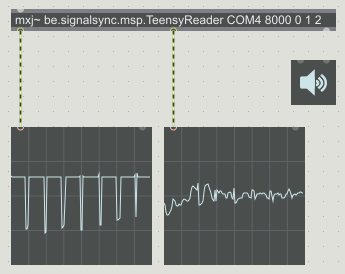
\includegraphics[width=0.4\textwidth]{TeensyReader.png}
	\end{center}
	\label{teensyReader}
\end{figure}

Figuur \ref{teensyReader} toont deze module waarbij de uitgaande verbindingen zijn aangesloten op scope objecten. Hierdoor wordt de data gevisualiseerd.

Een uitgebreide handleiding voor het gebruik van deze module is te vinden in bijlage X (TODO).
%TODO handleiding schrijven

\subsubsection{Implementatie}

Een Max/MSP module kan in Java geschreven worden door een klasse te laten overerven van \texttt{MSPPerformer}. Bij de constructie worden de \textit{outlets} (de uitgaande verbindingen) geïnitialiseerd en wordt er een \texttt{TeensyDAQ} object aangemaakt. Dit is een object uit afkomstig uit de \texttt{TeensyDAQ} bibliotheek ontwikkeld aan het IPEM. Deze bibliotheek biedt een low-level interface naar de Teensy microcontroller aan. Na het aanmaken van dit object registreert de module zich als \textit{handler}. Om dit mogelijk te maken wordt de methode \texttt{handle} van de interface \texttt{DAQDataHandler} geïmplementeerd. Na het registreren wordt deze methode consequent opgeroepen met samples afkomstig van de Teensy microcontroller. Deze samples worden vervolgens gebufferd.

Een klasse die overerft van \texttt{MSPPerformer} moet de methode \texttt{perform} implementeren. In deze methode worden de samples uit de buffers gehaald, geresamplet naar de Max/MSP samplefrequentie en verstuurd door de outlets.

\subsection{De synchronisatiemodule}

De tweede module zal de synchronisatie van de streams verzorgen en is geïmplementeerd in de klasse \texttt{Sync}. De module maakt gebruik van \texttt{RealtimeSignalSync} om de latencies tussen de audiostreams te bepalen. De module kan in Max/MSP met volgende code worden aangemaakt: \texttt{mxj\textapprox\  be.signalsync.msp.Sync <<parameter>>}

\subsubsection{Instellen van de stream structuur}

De module verwacht één parameter van het type \texttt{String} die beschrijft hoe de streams gestructureerd zijn. De structuur wordt voorgesteld als een door komma's gescheiden reeks van de letters 'a' en 'd'. Elk door deel bepaald de structuur van een \texttt{StreamGroup} waarin de letters 'a' en 'd' respectievelijk voor een audiostream en datastream staan. Per deel mag uiteraard maar eenmaal de letter 'a' voorkomen. De volledige tekenreeks  (de verzameling van alle \texttt{StreamGroups}) stelt de structuur van een \texttt{StreamSet} voor. Op basis van deze string worden de \texttt{Stream} objecten aangemaakt en onderverdeeld in \texttt{StreamGroups} en \texttt{StreamSets}.

Dit zou een mogelijke parameter voor deze module kunnen zijn: \texttt{addd,dad}. De eerste \texttt{StreamGroup} bestaat uit 4 streams waarbij de synchronisatie met de eerste stream zal worden uitgevoerd. De tweede \texttt{StreamGroup} bestaat uit 3 streams. De tweede stream stelt hierbij de audiostream voor.

Figuur \ref{maxStreamSync} toont hoe deze module gebruikt moet worden in combinatie met de \texttt{TeensyReader}. De audiostream \textit{outlets} (bepaald door de vierde parameter van de twee \texttt{TeensyReaders}) worden verbonden met de audiostream \textit{inlets} van de \texttt{Sync} module (bepaald door de letters 'a' van de parameter).

\begin{figure}[h!]
	\captionsetup{width=0.8\textwidth}
	\caption[Synchronisatie in Max/MSP]{De synchronisatie van streams in Max/MSP afkomstig van twee Teensy microcontrollers.}
	\begin{center}
		\advance\parskip0.3cm
		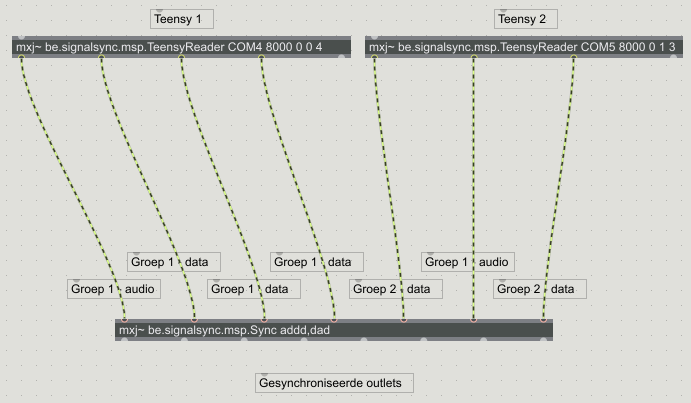
\includegraphics[width=\textwidth]{maxSync.png}
	\end{center}
	\label{maxStreamSync}
\end{figure}

\subsubsection{Implementatie}

Net zoals \texttt{TeensyReader} erft deze module over van \texttt{MSPPerformer}. Ook wordt de interface \texttt{SyncEventListener} geïmplementeerd. In de constructor wordt op basis van de parameter van de module een \texttt{StreamSet} bestaande uit \texttt{MSPStream} objecten aangemaakt. In de perform methode van de module worden de signaalvectoren doorgegeven aan de \texttt{MSPStream} objecten. De synchronisatie wordt verwezenlijkt door in de constructor een \texttt{RealtimeSignalSync} object aan te maken waarop de klasse zich registreert. Aan het \texttt{RealtimeSignalSync} object wordt de \texttt{StreamSet} meegegeven. Elke keer wanneer er informatie over de latency beschikbaar is wordt de methode \texttt{onSyncEvent} opgeroepen met alle latencies.

Met behulp van deze latencies moeten de binnenkomende Max/MSP datastreams gemanipuleerd worden zodat ze perfect synchroon lopen. Dit is in de laatste versie nog niet geïmplementeerd. In de huidige implementatie worden de latencies in de Max/MSP console geprint.





\chapter{Evaluatie}
\label{evaluatie}

Om de kwaliteit van de softwarebibliotheek te kunnen garanderen zijn er verschillende soorten testen uitgevoerd. 

De eerste soort testen zijn geschreven voor het bepalen en analyseren van de kwaliteit van de algoritmes. De algoritmes worden hierbij blootgesteld aan audiofragmenten waartussen de latency bepaalt moet worden. Met behulp van onder meer deze test zijn de optimale parameterwaarden bepaalt.

Buiten het testen van de algoritmes zijn er ook enkele unit testen geschreven voor het testen van enkele cruciale elementen van de softwarebibliotheek. Deze testen zijn cruciaal om het aantal bugs in de softwarelogica te beperken.

Het laatste deel van dit hoofdstuk zal dieper ingaan op de zaken die niet geïmplementeerd zijn maar die in de toekomst zeker een meerwaarde kunnen betekenen.

\section{Testen van de algoritmes}

Het testen van de algoritmes wordt uitgevoerd met behulp de JUnit testcase \texttt{SynchronizationTest} uit het package \texttt{be.signalsync.test}. Deze testcase laat toe om de slices van verschillende audiofragmenten met elkaar te matchen en te analyseren waar de algoritmes precies in de fout gaan.

\subsection{Aanmaken van de dataset}

Bij het uitvoeren van deze test is het de bedoeling om enkel de algoritmes te testen. Om niet afhankelijk te zijn van andere softwareonderdelen wordt de dataset op voorhand aangemaakt. Het aanmaken van deze dataset gebeurt in twee stappen. Eerst wordt het originele audiofragment gewijzigd door er bijvoorbeeld latency aan toe te voegen. Dit gebeurt met behulp van een Perl script. Vervolgens worden de verschillende audiofragmenten in slices geknipt en opgeslagen. In de testcase worden de algoritmes rechtstreeks op deze slices uitgevoerd zonder andere softwareonderdelen aan te roepen.

\subsection{Toevoegen van latency}

In het meest eenvoudige scenario wordt de latency berekend tussen twee identieke audiofragmenten waarbij er één audiofragment bewerkt is door stilte toe te voegen of een stukje weg te knippen. Aangezien de audiofragmenten buiten deze wijziging identiek zijn zouden de algoritmes in theorie geen enkele fout mogen maken.

Voor de test worden 13 varianten voorzien van een audiofragment. Het originele audiofragment is de referentie. Er zijn zowel varianten met een positieve latency als varianten met een negatieve latency voorzien.

De resultaten van de test bevinden zich in bijlage \ref{appendix-b}. Het accoustic fingerprinting heeft de verschillende testen foutloos doorstaan. Het kruiscovariantie algoritme maakte echter enkele fouten wanneer de test maar eenmaal wordt uitgevoerd. Dit is logisch te verklaren. Het kruiscovariantie wordt namelijk uitgevoerd op een zeer klein stukje audio. Wanneer de test maar eenmaal wordt uitgevoerd kan het gebeuren dat één van de buffers toevallig enkel stilte bevat (alle samples hebben de waarde 0.0). In dat geval is de kruiscovariantie voor elke verschuiving 0 en wordt er hoogst waarschijnlijk een fout resultaat teruggegeven. Dit probleem kan gemakkelijk opgelost worden door het algoritme minstens 2 keer uit te voeren (zie \ref{crosscovariance-repeated}).

\subsection{Toevoegen van een sinusgolf}

In sectie \ref{crosscovariance-repeated} is geschreven dat het kruiscovariantie algoritme het moeilijk krijgt wanneer de te matchen geluidsgolven visueel erg van elkaar verschillen. Dit wordt gesimuleerd door het toevoegen van een lage toon (sinusgolf van $50Hz$ en $100Hz$) aan één van de audiofragmenten. Door het kruiscovariantie algoritme verschillende keren uit te voeren wordt de invloed van dit probleem beperkt.

De resultaten uit bijlage \ref{appendix-c} tonen aan dat het meerdere malen uitvoeren van het algoritme wel degelijk betere resultaten levert. Bij het laatste experiment (waarbij het algoritme 20 maal werd uitgevoerd) werden alle latencies correct bepaald.

\section{Praktijktesten}

\section{Testen van de softwarecomponenten}



\section{Mogelijke verbeteringen}


\chapter{Conclusie}

In dit hoofdstuk zal worden teruggeblikt naar wat er in dit onderzoek precies verwezenlijkt is. In sectie \ref{doel-masterproef} is er omschreven welke zaken er ontwikkeld zouden moeten worden om deze masterproef als geslaagd te kunnen beschouwen. In sectie \ref{evaluatie-criteria} worden de vereisten omtrent de snelheid en precisie van de algoritmes verder uitgediept. Elk omschreven doel of criteria zal in dit hoofdstuk worden getoetst aan de op dit moment beschikbare implementatie.

\section{Doelen}

Het eerste doel uit \ref{doel-masterproef} stelt dat de algoritmes aangepast en/of geoptimaliseerd moeten worden zodat ze de latency tussen audiofragmenten opgenomen met een basic microfoon kunnen bepalen tot op minstens één milliseconde nauwkeurig. De praktijktest beschreven in \ref{praktijktest} toont aan dat dit mogelijk is.

Het tweede doel is de implementatie van de softwarebibliotheek. Met behulp van deze bibliotheek moet het mogelijk zijn om programmatisch streams te kunnen aanmaken en synchroniseren. Het ontwerp van deze softwarebibliotheek is omschreven in \ref{ontwerp}. Dit toont aan dat het doel ook is verwezenlijkt.

Het derde doel is grotendeels afgewerkt. De gebruikersinterface kan door musicologen zelf worden samengesteld door gebruik te maken van Max/MSP. In de praktijktest is aangetoond dat het mogelijk is om streams in te lezen en de latency tussen de streams te bepalen. Het enige wat nog geïmplementeerd moet worden is het daadwerkelijk gesynchroniseerd wegschrijven van de streams.

\section{Beoordelingscriteria algoritmes}

In \ref{evaluatie-criteria} werden enkele meer specifieke criteria opgelegd waaraan de synchronisatie moet voldoen.

Het eerste criterium stelt dat het mogelijk moet zijn om met een buffergrootte (de grootte van de slices) van maximaal 10 seconden de synchronisatie uit te voeren. De testen omschreven in \ref{algoritme-test} en \ref{praktijktest} zijn uitgevoerd met de vooropgestelde buffergrootte en zijn geslaagd. Het huidige systeem voldoet dus aan dit criterium.

Het tweede criterium bepaalt de snelheid waarmee gedropte samples gedetecteerd kunnen worden. In de fase van het onderzoek waarin deze criteria zijn opgesteld was het nog onduidelijk welke factoren hier allemaal invloed op hebben. In sectie \ref{streambuffers} is onder meer omschreven welke invloed de grootte en stapgrootte van de buffers hebben op de detectiesnelheid. Ook het eventueel filteren van de resultaten (beschreven in \ref{filtering}) heeft een invloed op de detectiesnelheid. De testen die in hoofdstuk \ref{evaluatie} omschreven werden voldoen aan de vooropgestelde maximale detectiesnelheid van 10 seconden. Er werd namelijk een slicegrootte van 10 seconden en stapgrootte van 5 seconde gehanteerd. Deze maximale detectiesnelheid kan met deze instellingen niet worden bereikt indien er aan foutcorrectie wordt gedaan.

Het laatste criterium stelt dat het mogelijk moet zijn om drift te detecteren. De detectiesnelheid hiervan is gelijk aan de snelheid waarmee gedropte samples gedetecteerd kunnen worden. In de praktijktest trad dit verschijnsel op. Het is bijgevolg bewezen dat dit mogelijk is.

% appendices
\begin{appendices}
	\chapter{Resultaten: DTW experiment}
\label{appendix-a}

In dit experiment proberen we de nauwkeurigheid van het DTW algoritme te bepalen wanneer streams gebufferd worden. Hiertoe bepaalden we eerst de latency tussen twee audiofragmenten. Vervolgens verkleinden we iteratief de duur van het fragment met 10 seconden waarop we het algoritme opnieuw uitvoerden. Tenslotte vergeleken we de buffergrootte en nauwkeurigheid van de resultaten.

We hebben gebruik gemaakt van twee audiofragmenten waarbij het ene fragment 2.390 seconden vertraging heeft ten opzichte van het andere fragment. Beide fragmenten hebben samplefrequentie van 8000 Hz. Eén van de twee fragmenten is een opname van het origineel en bijgevolg van matige kwaliteit.

Het experiment is uitgevoerd in \textit{Sonic Visualiser} met behulp van de \textit{Match Performance Aligner} plug-in. Deze plug-in laat synchronisatie toe met behulp van het DTW algoritme. De implementatie wordt uitgebreider besproken in artikel \cite{dixon2005match}. Voor dit experiment hebben we de default instellingen gebruikt. De plug-in bepaalt elke twintig milliseconden de latency tussen beide fragmenten.

De volgende tabel geeft de resultaten van het experiment weer. De eerste kolom bevat de lengte van de vergeleken fragmenten in seconden. Deze lengte stelt de buffergrootte voor van een audiostream. De tweede kolom geeft aan hoeveel seconden van de stream moet worden verwerkt tot er een stabiel resultaat wordt bekomen. De derde kolom geeft het gemitdoddelde weer van de gevonden latencies. Deze waarde wordt berekend vanaf dat het algoritme een stabiel resultaat heeft gevonden. De vierde kolom bevat de standaardafwijking van dit resultaat.\\

\begin{center}
\begin{tabular}{ c  c  c  c }
	\hline
	\textbf{Lengte} & \textbf{Tijd tot stabiel} & \textbf{Gemiddelde latency} & \textbf{Standaardafwijking} \\
	\hline
	60s & 2.540s & 2,393s & 0.048s \\
	50s & 2.540s & 2,390s & 0.095s \\
	40s & 2.540s & 2,394s & 0.020s \\
	30s & 2.540s & 2,384s & 0.145s \\
	20s & 2.540s & 2,390s & 0.108s \\
	10s & 2.540s & 2,395s & 0.025s \\
	\\
\end{tabular}\\
\end{center}

Uit bovenstaande resultaten kunnen we verschillende zaken concluderen. Ten eerste zien we aan de standaardafwijking dat de individuele resultaten (die iedere 20ms gegenereerd worden) niet nauwkeurig genoeg zijn om te gebruiken in onze toepassing. De gemiddelde waarde komt wel in de buurt van de werkelijke latency maar is nog steeds niet zo nauwkeurig. Ook moeten we bij de berekening van het gemiddelde rekening houden met het feit dat het algoritme pas na een bepaalde tijd een stabiel resultaat vindt, in dit geval 2.540s.

We hebben dit algoritme ook uitgetest op een fragment waaruit 500 ms hebben weggeknipt om het probleem met gedropte samples te simuleren. Het algoritme reageerde hier zeer snel op: de nieuwe latency werd na 240 ms gevonden. Het probleem is dat we zojuist hebben getracht de nauwkeurigheid te verbeteren door het gemiddelde te nemen van de resultaten. Dit heeft als gevolg dat wanneer er samples gedropt zijn het eindresultaat zich bevindt tussen de initiële en nieuwe latency.


\end{appendices}
% Bibliografie toevoegen
\bibliographystyle{plainnat}
\bibliography{../bronnen/bronnen}

\backmatter

%Lijst van figuren toevoegen, en toevoegen aan inhoudstabel
\listoffigures
\addcontentsline{toc}{chapter}{Lijst van figuren}

%Lijst van tabellen toevoegen, en toevoegen aan inhoudstabel
\listoftables
\addcontentsline{toc}{chapter}{Lijst van tabellen}

%Lijst van codefragmenten toevoegen, en toevoegen aan inhoudstabel
\lstlistoflistings
\addcontentsline{toc}{chapter}{Lijst van codefragmenten}

% lege pagina (!!)

% kaft

\end{document}
